%! Mode:: "TeX:UTF-8"
%! TEX program = xelatex
\PassOptionsToPackage{quiet}{xeCJK}
\documentclass[withoutpreface,bwprint]{cumcmthesis}
\usepackage{etoolbox}
\BeforeBeginEnvironment{tabular}{\zihao{-5}}
\usepackage[numbers,sort&compress]{natbib}  % 文献管理宏包
\usepackage[framemethod=TikZ]{mdframed}  % 框架宏包
\usepackage{url}  % 网页链接宏包
\usepackage{subcaption}  % 子图宏包
\newcolumntype{C}{>{\centering\arraybackslash}X}
\newcolumntype{R}{>{\raggedleft\arraybackslash}X}
\newcolumntype{L}{>{\raggedright\arraybackslash}X}

\usepackage{multirow}
\usepackage{array}

\title{全国大学生数学建模竞赛论文模板}  % 论文标题
\tihao{}  % 题号
\baominghao{}  % 报名号
\schoolname{}  % 学校
\membera{}  % 队员a
\memberb{}  % 队员b
\memberc{}  % 队员c
\supervisor{}  % 指导老师
\yearinput{}
\monthinput{}
\dayinput{}

%%%%%%%%%%%%%%%%%%%%%%%%%%%%%%%%%%%%%%%%%%%%%%%%%%%%%%%%%%%%%
%% 正文
\begin{document}
\begin{samepage}
\begin{center}
\renewcommand{\arraystretch}{2}
\begin{tabular}{|>{\centering\arraybackslash}m{0.13\textwidth}
                |>{\centering\arraybackslash}m{0.65\textwidth}
                |>{\centering\arraybackslash}m{0.17\textwidth}|}
    \hline
    \songti 所属类别
    & \multirow{2}{*}{\centering\songti\zihao{4} \textbf{2024年“华数杯”全国大学生数学建模竞赛}}
    & \songti 参赛编号 \\
    \cline{1-1} \cline{3-3}
    \songti 本科组 & & CM2400947 \\
    \hline
\end{tabular}
\end{center}

\maketitle

\begin{abstract}
    母亲的身心健康对婴儿的早期成长和发展具有重要影响。已有研究表明,母亲的身体状况以及心理健康(如压力、抑郁、焦虑等)不仅关系到婴儿的生理健康,还会影响婴儿的认知、情感、社会行为等多方面成长。婴儿的行为特征和睡眠质量常常作为衡量婴儿发展状况的重要指标。基于这方面的专业背景,本文对相关影响机制进行了研究与建模。
    
    \textbf{对于问题一,}本文通过分析390名婴儿及其母亲的身体和心理相关指标数据,研究了母亲因素对婴儿行为特征和睡眠质量的影响关系。
    
    \textbf{对于问题二,}基于婴儿行为问卷,将婴儿行为特征划分为安静型、中等型和矛盾型,建立了行为特征与母亲身体、心理指标之间的数学关系模型,并利用该模型预测了20组缺失婴儿行为类型。
    
    \textbf{对于问题三,}建立了CBTS、EPDS、HADS评分与治疗费用的关联模型,针对编号238的矛盾型婴儿,分析通过最小治疗费用使其行为特征由矛盾型转变为中等型和安静型的策略及调整路径。
    
    \textbf{对于问题四,}选取婴儿睡眠的多项指标,综合评判睡眠质量,并建立母亲各项指标与婴儿综合睡眠质量的关联模型,进而预测缺失数据婴儿的睡眠类别。
    
    最后,结合模型结果,对如何提升238号婴儿的睡眠质量等级为优提出了具体的治疗方案和优化建议。
    
    \keywords{母亲心理健康\quad  婴儿成长\quad  行为特征\quad  睡眠质量 \quad 数学建模}
    \end{abstract}
\end{samepage}
%%%%%%%%%%%%%%%%%%%%%%%%%%%%%%%%%%%%%%%%%%%%%%%%%%%%%%%%%%%%% 

% \tableofcontents  % 目录
% \newpage

%%%%%%%%%%%%%%%%%%%%%%%%%%%%%%%%%%%%%%%%%%%%%%%%%%%%%%%%%%%%%  
\section{问题重述}
\subsection{问题背景}
问题背景

%%%%%%%%%%%%%%%%%%%%%%%%%%%%%%%%%%%%%%%%%%%%%%%%%%%%%%%%%%%%% 

\subsection{问题要求}

\textbf{问题1}  

\textbf{问题2}  

\textbf{问题3} 

\textbf{问题4}  

%%%%%%%%%%%%%%%%%%%%%%%%%%%%%%%%%%%%%%%%%%%%%%%%%%%%%%%%%%%%% 

\section{问题分析}
\subsection{问题一分析}
对于问题一,

\subsection{问题二分析}	
对于问题二,

\subsection{问题三分析}
对于问题三,

\subsection{问题四分析}
对于问题四,

%%%%%%%%%%%%%%%%%%%%%%%%%%%%%%%%%%%%%%%%%%%%%%%%%%%%%%%%%%%%% 

\section{模型假设}

为简化问题,本文做出以下假设:

\begin{itemize}[itemindent=2em]
\item 假设1
\item 假设2
\item 假设3
\end{itemize}

%%%%%%%%%%%%%%%%%%%%%%%%%%%%%%%%%%%%%%%%%%%%%%%%%%%%%%%%%%%%% 

\section{符号说明}
\begin{table}[H]
\centering
\begin{tabularx}{\textwidth}{CLC}
\toprule
符号    & 说明    & 单位 \\
\midrule
$m     $& 质量 & $kg$ \\
$V     $& 体积 & $m^3$ \\
\bottomrule
\end{tabularx}
\label{tab:符号说明}
\end{table}


%%%%%%%%%%%%%%%%%%%%%%%%%%%%%%%%%%%%%%%%%%%%%%%%%%%%%%%%%%%%% 

%%%%%%%%%%%%%%%%%%%%%%%%%%%%%%%%%%%%%%%%%%%%%%%%%%%%%%%%%%%%% 

%%%%%%%%%%%%%%%%%%%%%%%%%%%%%%%%%%%%%%%%%%%%%%%%%%%%%%%%%%%%% 

%%%%%%%%%%%%%%%%%%%%%%%%%%%%%%%%%%%%%%%%%%%%%%%%%%%%%%%%%%%%% 

%%%%%%%%%%%%%%%%%%%%%%%%%%%%%%%%%%%%%%%%%%%%%%%%%%%%%%%%%%%%% 

\section{问题一的模型的建立和求解}


\subsection{数据预处理与特征工程}
高质量的数据是构建有效模型的基础。针对原始数据集,我们进行了以下关键的数据预处理和特征工程步骤,旨在确保数据的规范性、一致性和可用性,为后续的模型构建奠定坚实基础:

\subsubsection{睡眠时间格式转换}
原始数据中婴儿“整晚睡眠时间”以“HH:MM”字符串格式记录,且存在“99:99”等异常值。我们将其统一转换为浮点数表示的小时数,并对异常值进行了妥善处理,通常将其视为缺失值或根据业务逻辑进行填充。
$$ \text{时间}_{\text{小时}} = \text{小时} + \frac{\text{分钟}}{60} $$
此转换确保了睡眠时间数据的数值化和可计算性,使其能够被回归模型有效利用。

\subsubsection{分类变量编码与映射}
数据集中包含婚姻状况、教育程度、分娩方式、婴儿性别、入睡方式和婴儿行为特征等分类变量。为使其能够被回归模型处理,我们进行了以下操作:我们将原始的数值编码(如1、2、3等)映射为更具可读性的类别标签(如“未婚”、“已婚”;“哄睡法”、“自主入睡”)。对于无序的分类变量,如入睡方式、教育程度等,我们采用了独热编码将其转换为二元(0/1)指示变量。这有效避免了将分类变量误解释为有序数值,并消除了因任意数值赋值而引入的潜在偏差。例如,教育程度的“研究生”类别将被转换为一个独立的二元特征。值得一提的是,婴儿行为特征作为因变量,被映射为数值(如安静型=0,中等型=1,矛盾型=2),以适应多项逻辑回归模型的输入要求。

\subsubsection{数值型特征标准化}
对于母亲年龄、妊娠时间、CBTS、EPDS、HADS等数值型预测变量,我们均采用了标准差标准化(Z-score normalization)处理。
$$ X' = \frac{X - \mu}{\sigma} $$
其中,$X$ 是原始特征值,$\mu$ 是特征的均值,$\sigma$ 是特征的标准差。标准化后的特征均值为0,标准差为1。此步骤至关重要,它有助于消除不同特征因量纲和取值范围差异带来的影响,确保模型优化过程中所有特征得到同等重视;加速模型收敛,尤其对于基于梯度下降的优化算法(如逻辑回归);提高模型的可解释性和稳定性,避免某些特征因数值过大而主导模型。这些预处理步骤共同确保了数据的规范性、一致性和可用性,为后续的模型构建奠定了坚实基础。

\subsection{探索性数据分析 (EDA) 结果}
在正式构建模型之前,我们进行了全面的探索性数据分析,旨在揭示数据内部的结构、变量分布及其潜在关联,为后续模型选择与构建提供数据驱动的依据。

\subsubsection{变量分布特征}
我们首先对关键变量的分布特性进行了细致的探究,以全面了解数据的内在结构。
对母亲的心理指标(CBTS、EPDS和HADS得分)进行分析,如图1所示,这些指标的分布均呈现出明显的右偏态势。这清晰地表明,虽然研究样本中大部分母亲的心理健康状况总体良好,但仍有一部分母亲的得分相对较高,提示着她们可能存在不同程度的心理健康风险,需要进一步关注。

% 将图表移动到首次引用之后
\begin{figure}[htbp]
    \centering
    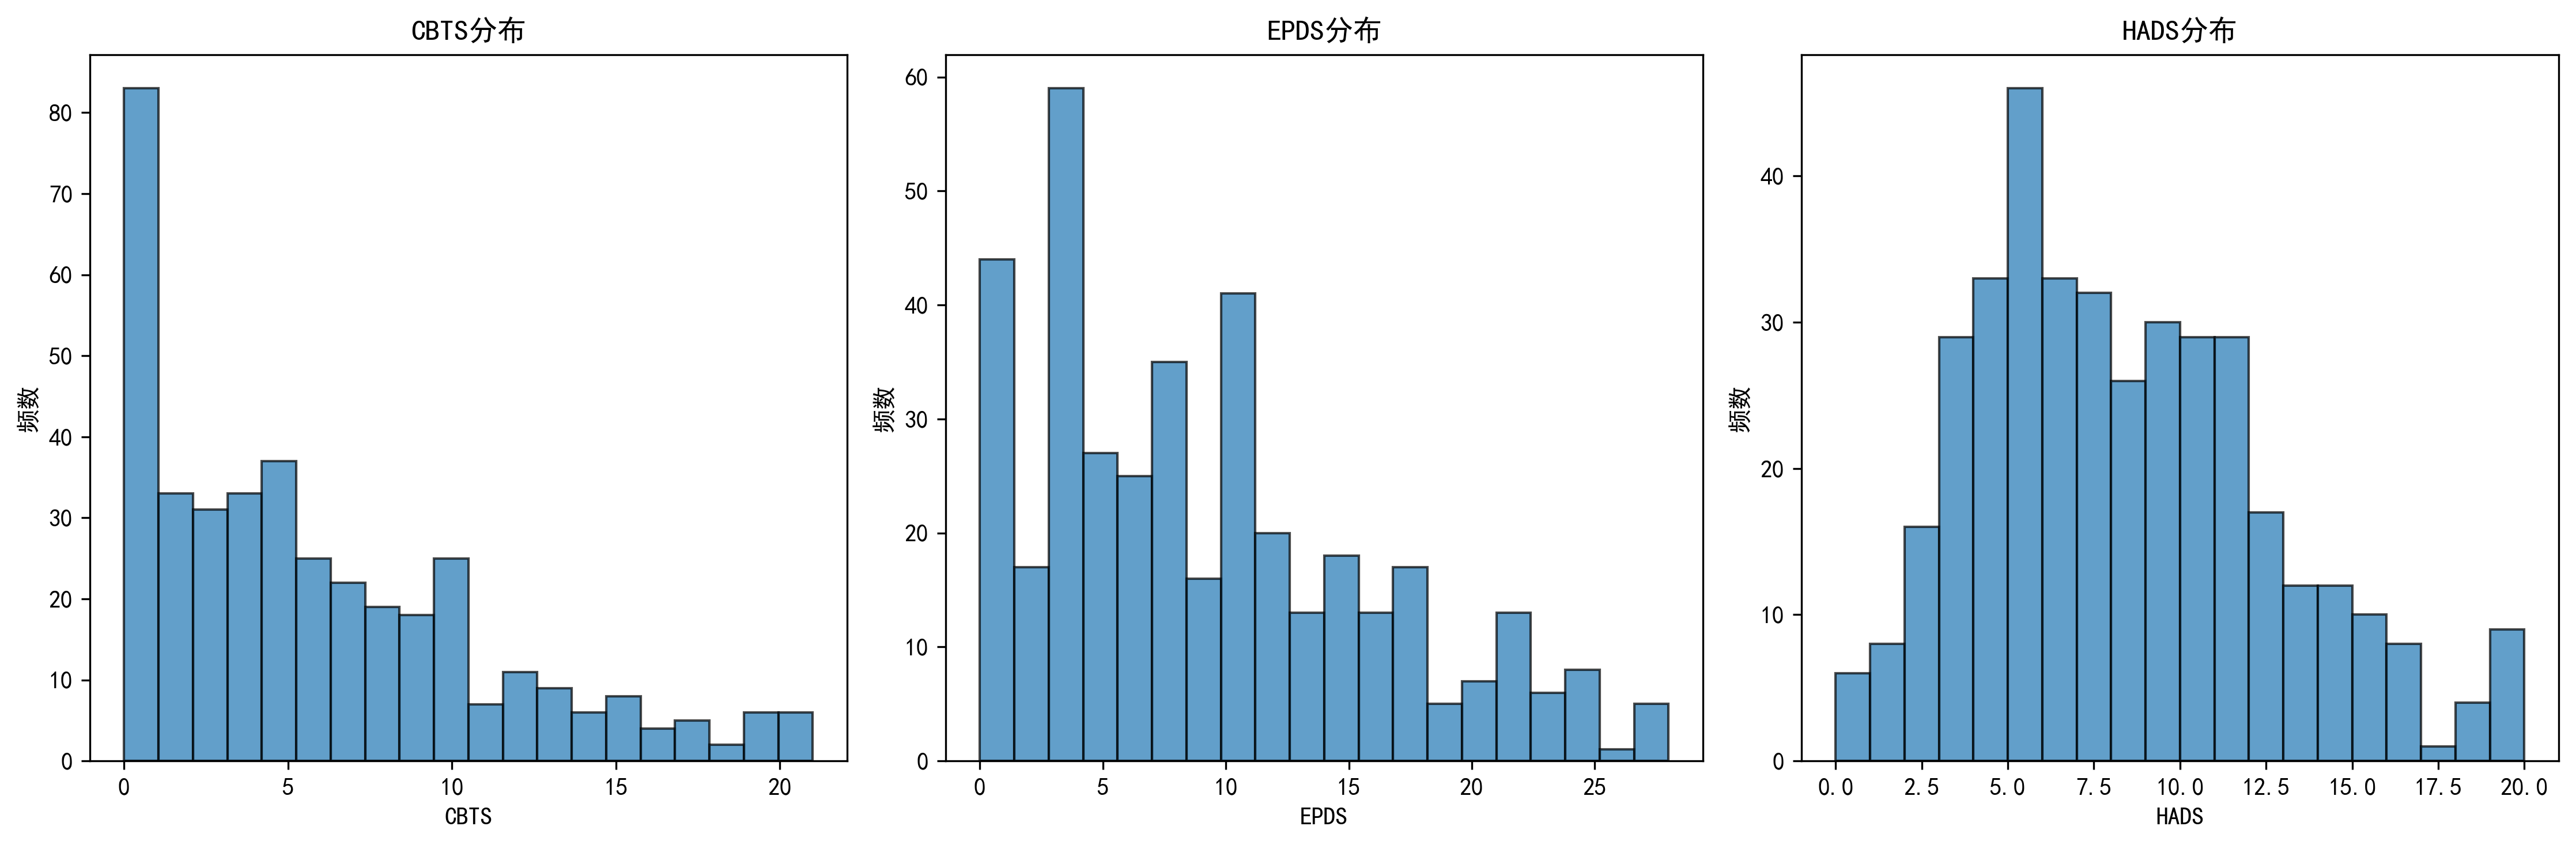
\includegraphics[width=0.9\textwidth]{figures/psychological_indicators_distribution.png}
    \caption{母亲心理指标分布}
    \label{fig:psychological_indicators_distribution}
\end{figure}

关于婴儿的睡眠质量,如图2所示,我们观察到婴儿的整晚睡眠时间主要集中在10至12小时这一区间,这与该年龄段婴儿正常的生理睡眠需求是基本吻合的。然而,在夜间睡醒次数方面,虽然大多数婴儿的醒来次数维持在0至2次,但数据中也包含少数夜间醒来频率较高的婴儿,这可能暗示了其睡眠模式存在潜在的改善空间。

% 将图表移动到首次引用之后
\begin{figure}[htbp]
    \centering
    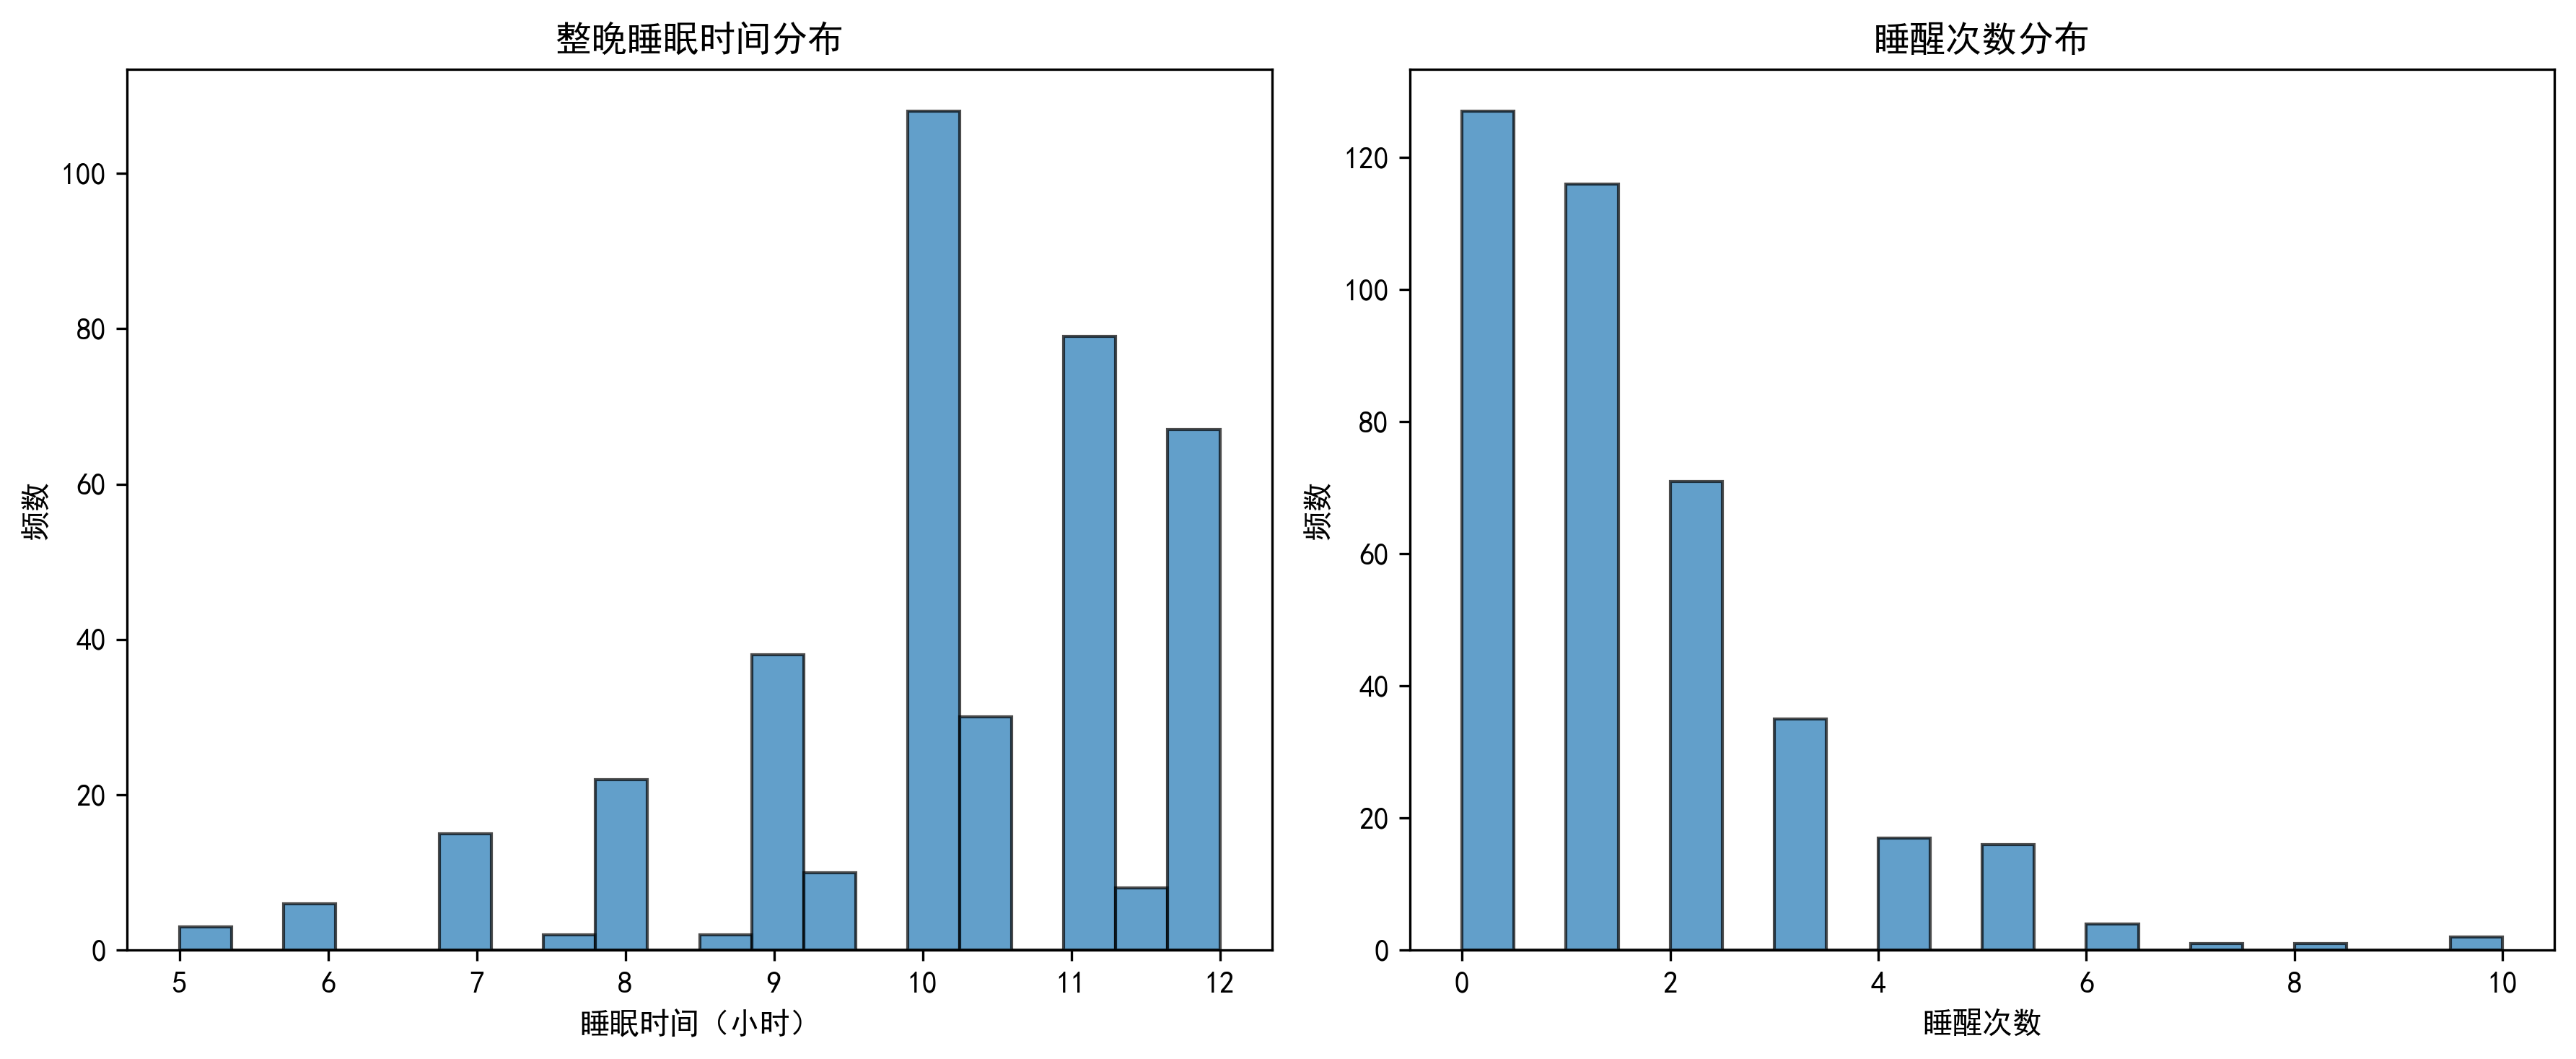
\includegraphics[width=0.8\textwidth]{figures/sleep_quality_distribution.png}
    \caption{睡眠质量指标分布}
    \label{fig:sleep_quality_distribution}
\end{figure}

如图3所示,婴儿行为特征的分布呈现出显著的不均衡性。其中,“中等型”婴儿在样本中占据了最大比例(57.7\%),其次是“安静型”婴儿(30.8\%),而“矛盾型”婴儿的比例最低,仅为11.5\%。这种类别分布的明显差异,在后续构建模型时需要予以特别考量,以确保模型不会因数据不平衡而产生偏差。

% 将图表移动到首次引用之后
\begin{figure}[htbp]
    \centering
    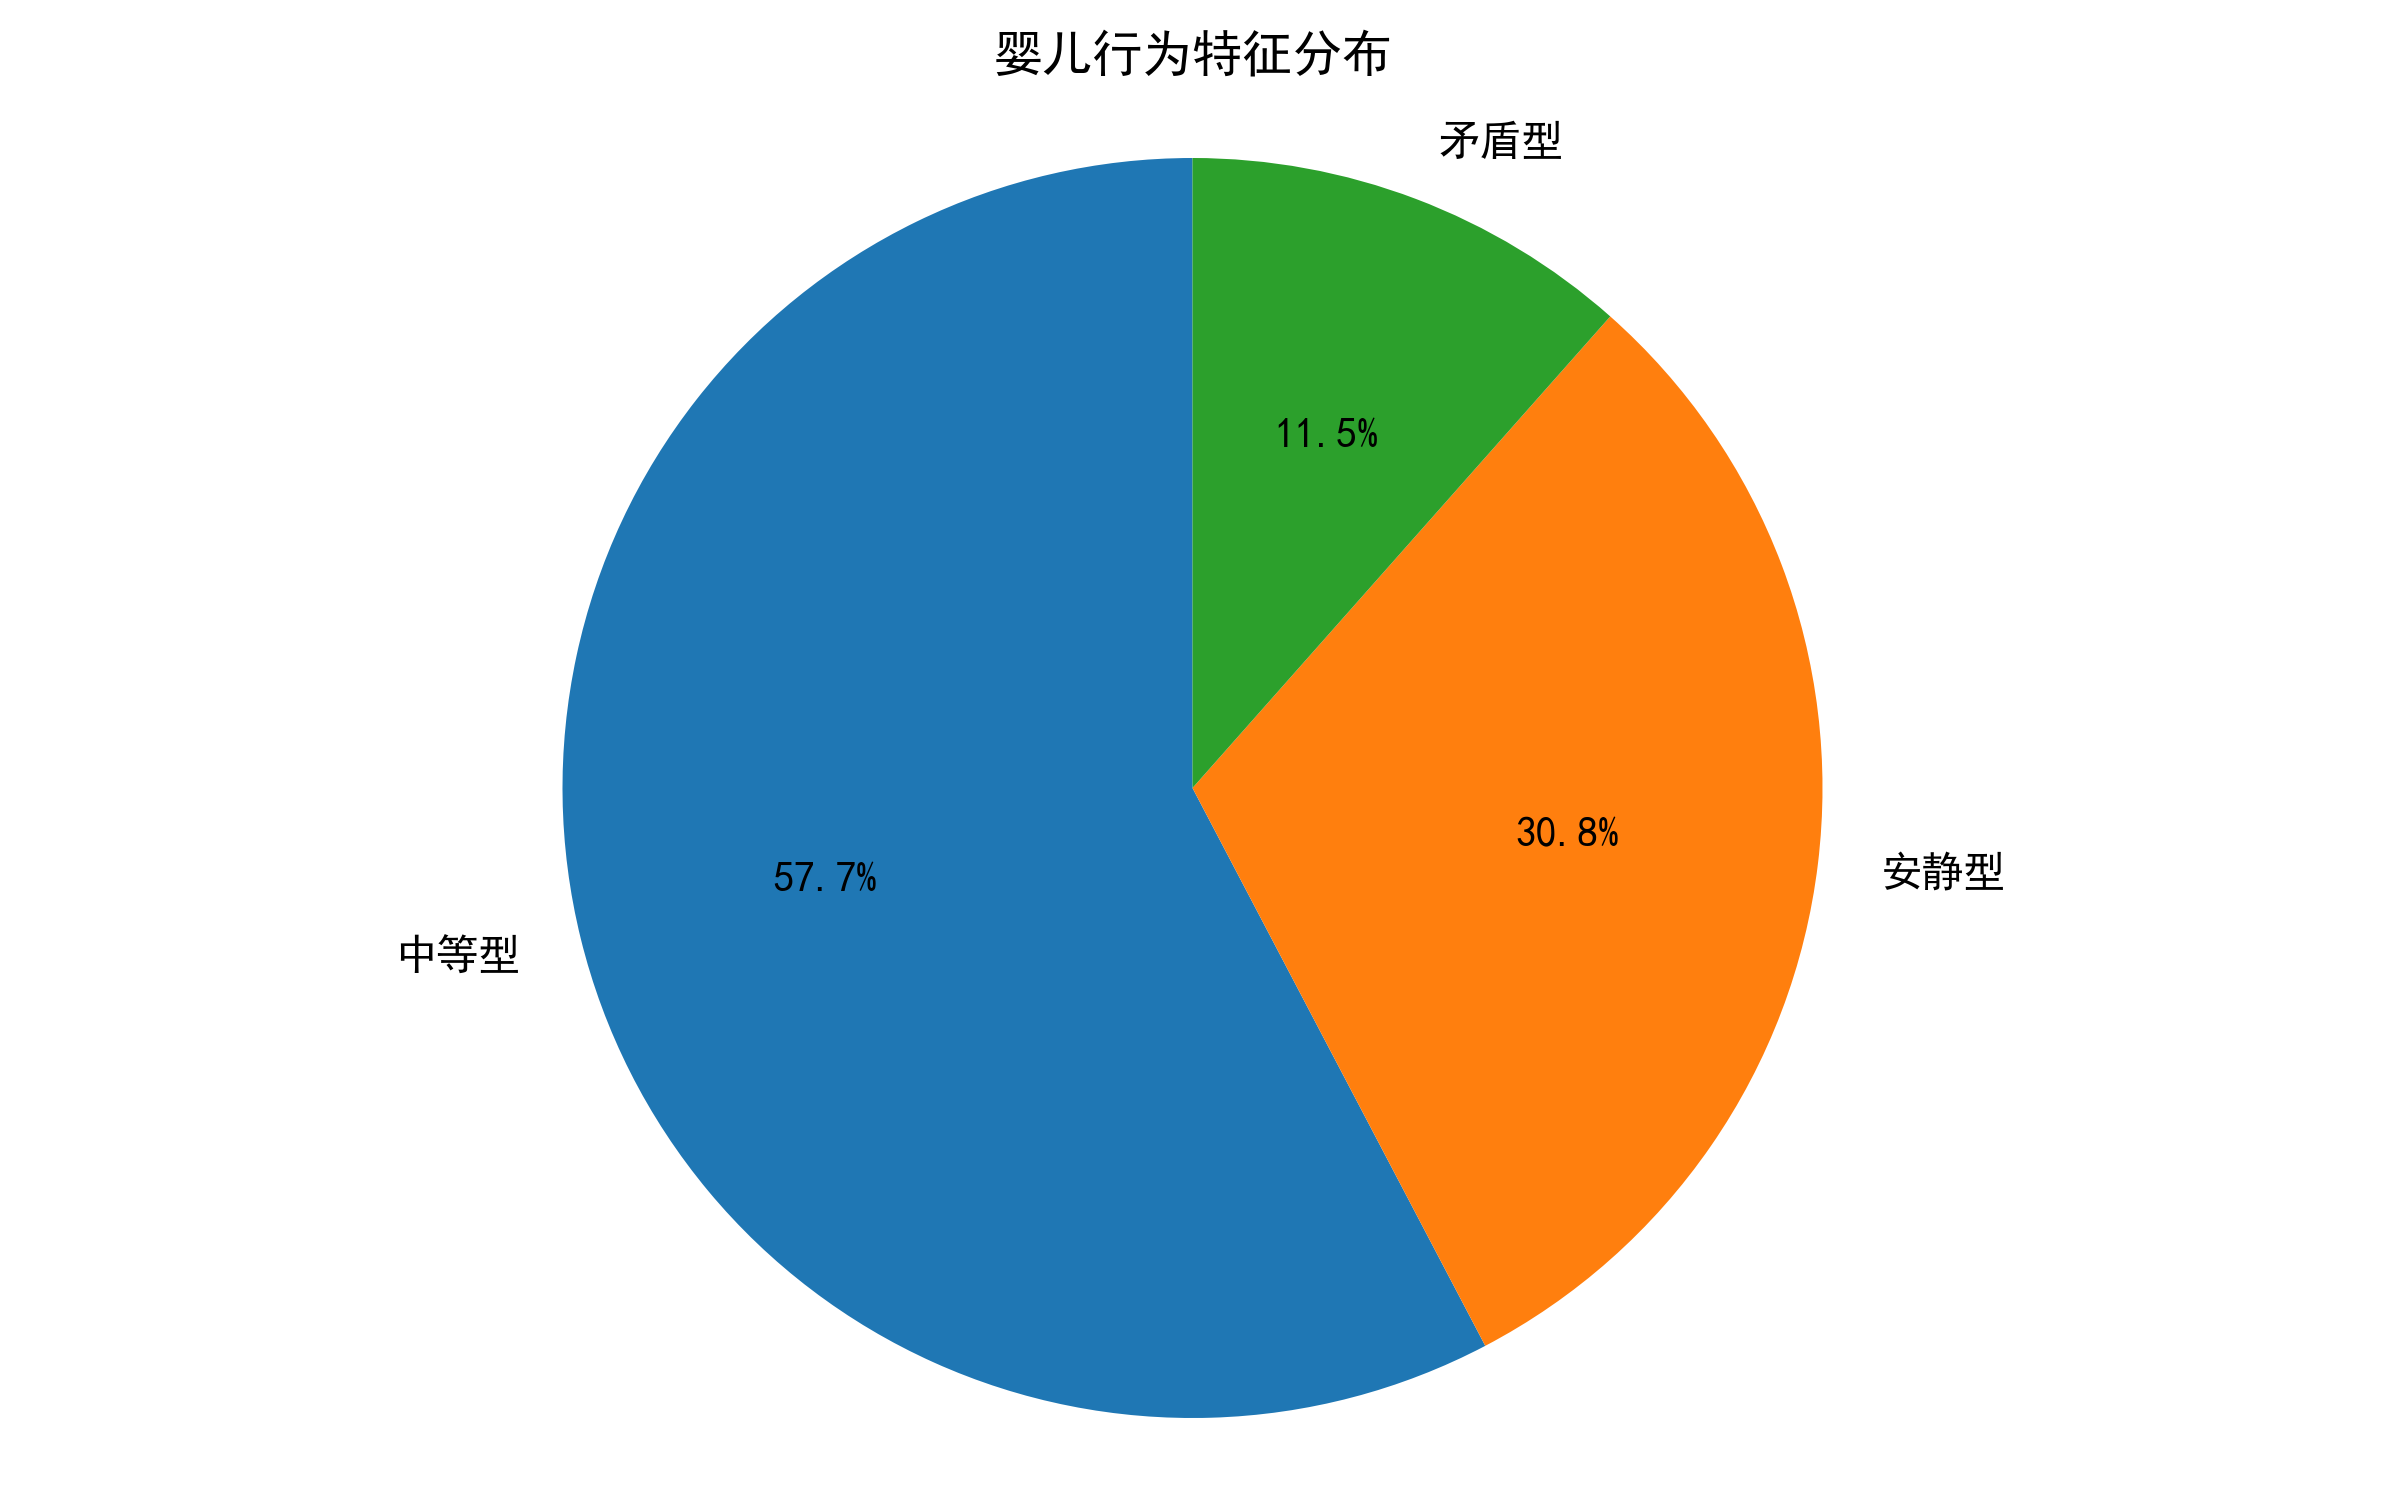
\includegraphics[width=0.5\textwidth]{figures/baby_behavior_distribution.png}
    \caption{婴儿行为特征分布}
    \label{fig:baby_behavior_distribution}
\end{figure}

\subsubsection{相关性分析}
为了洞察各数值型变量之间的相互关系,我们计算了皮尔逊相关系数,并以热力图形式直观展示了其关联强度。
我们发现母亲的EPDS与HADS得分之间存在高达0.79的强相关性,CBTS与EPDS为0.78,而CBTS与HADS也达到0.69。这种高度的正相关性强烈表明,抑郁、焦虑以及创伤后应激障碍等心理困扰并非孤立存在,而是倾向于同时出现,这为临床干预策略的制定提供了重要启示,即应采取综合性的评估与治疗方法。
分析进一步揭示,如图\ref{fig:correlation_heatmap}所示,母亲的各项心理指标(CBTS、EPDS、HADS)与婴儿的整晚睡眠时间呈现弱到中等程度的负相关,而与夜间睡醒次数则呈正相关。这一发现初步勾勒出母亲心理压力水平越高,婴儿睡眠质量可能越差的变化规律,突显了母亲心理健康对婴儿健康发展的重要影响。

% 将图表移动到首次引用之后
\begin{figure}[htbp]
    \centering
    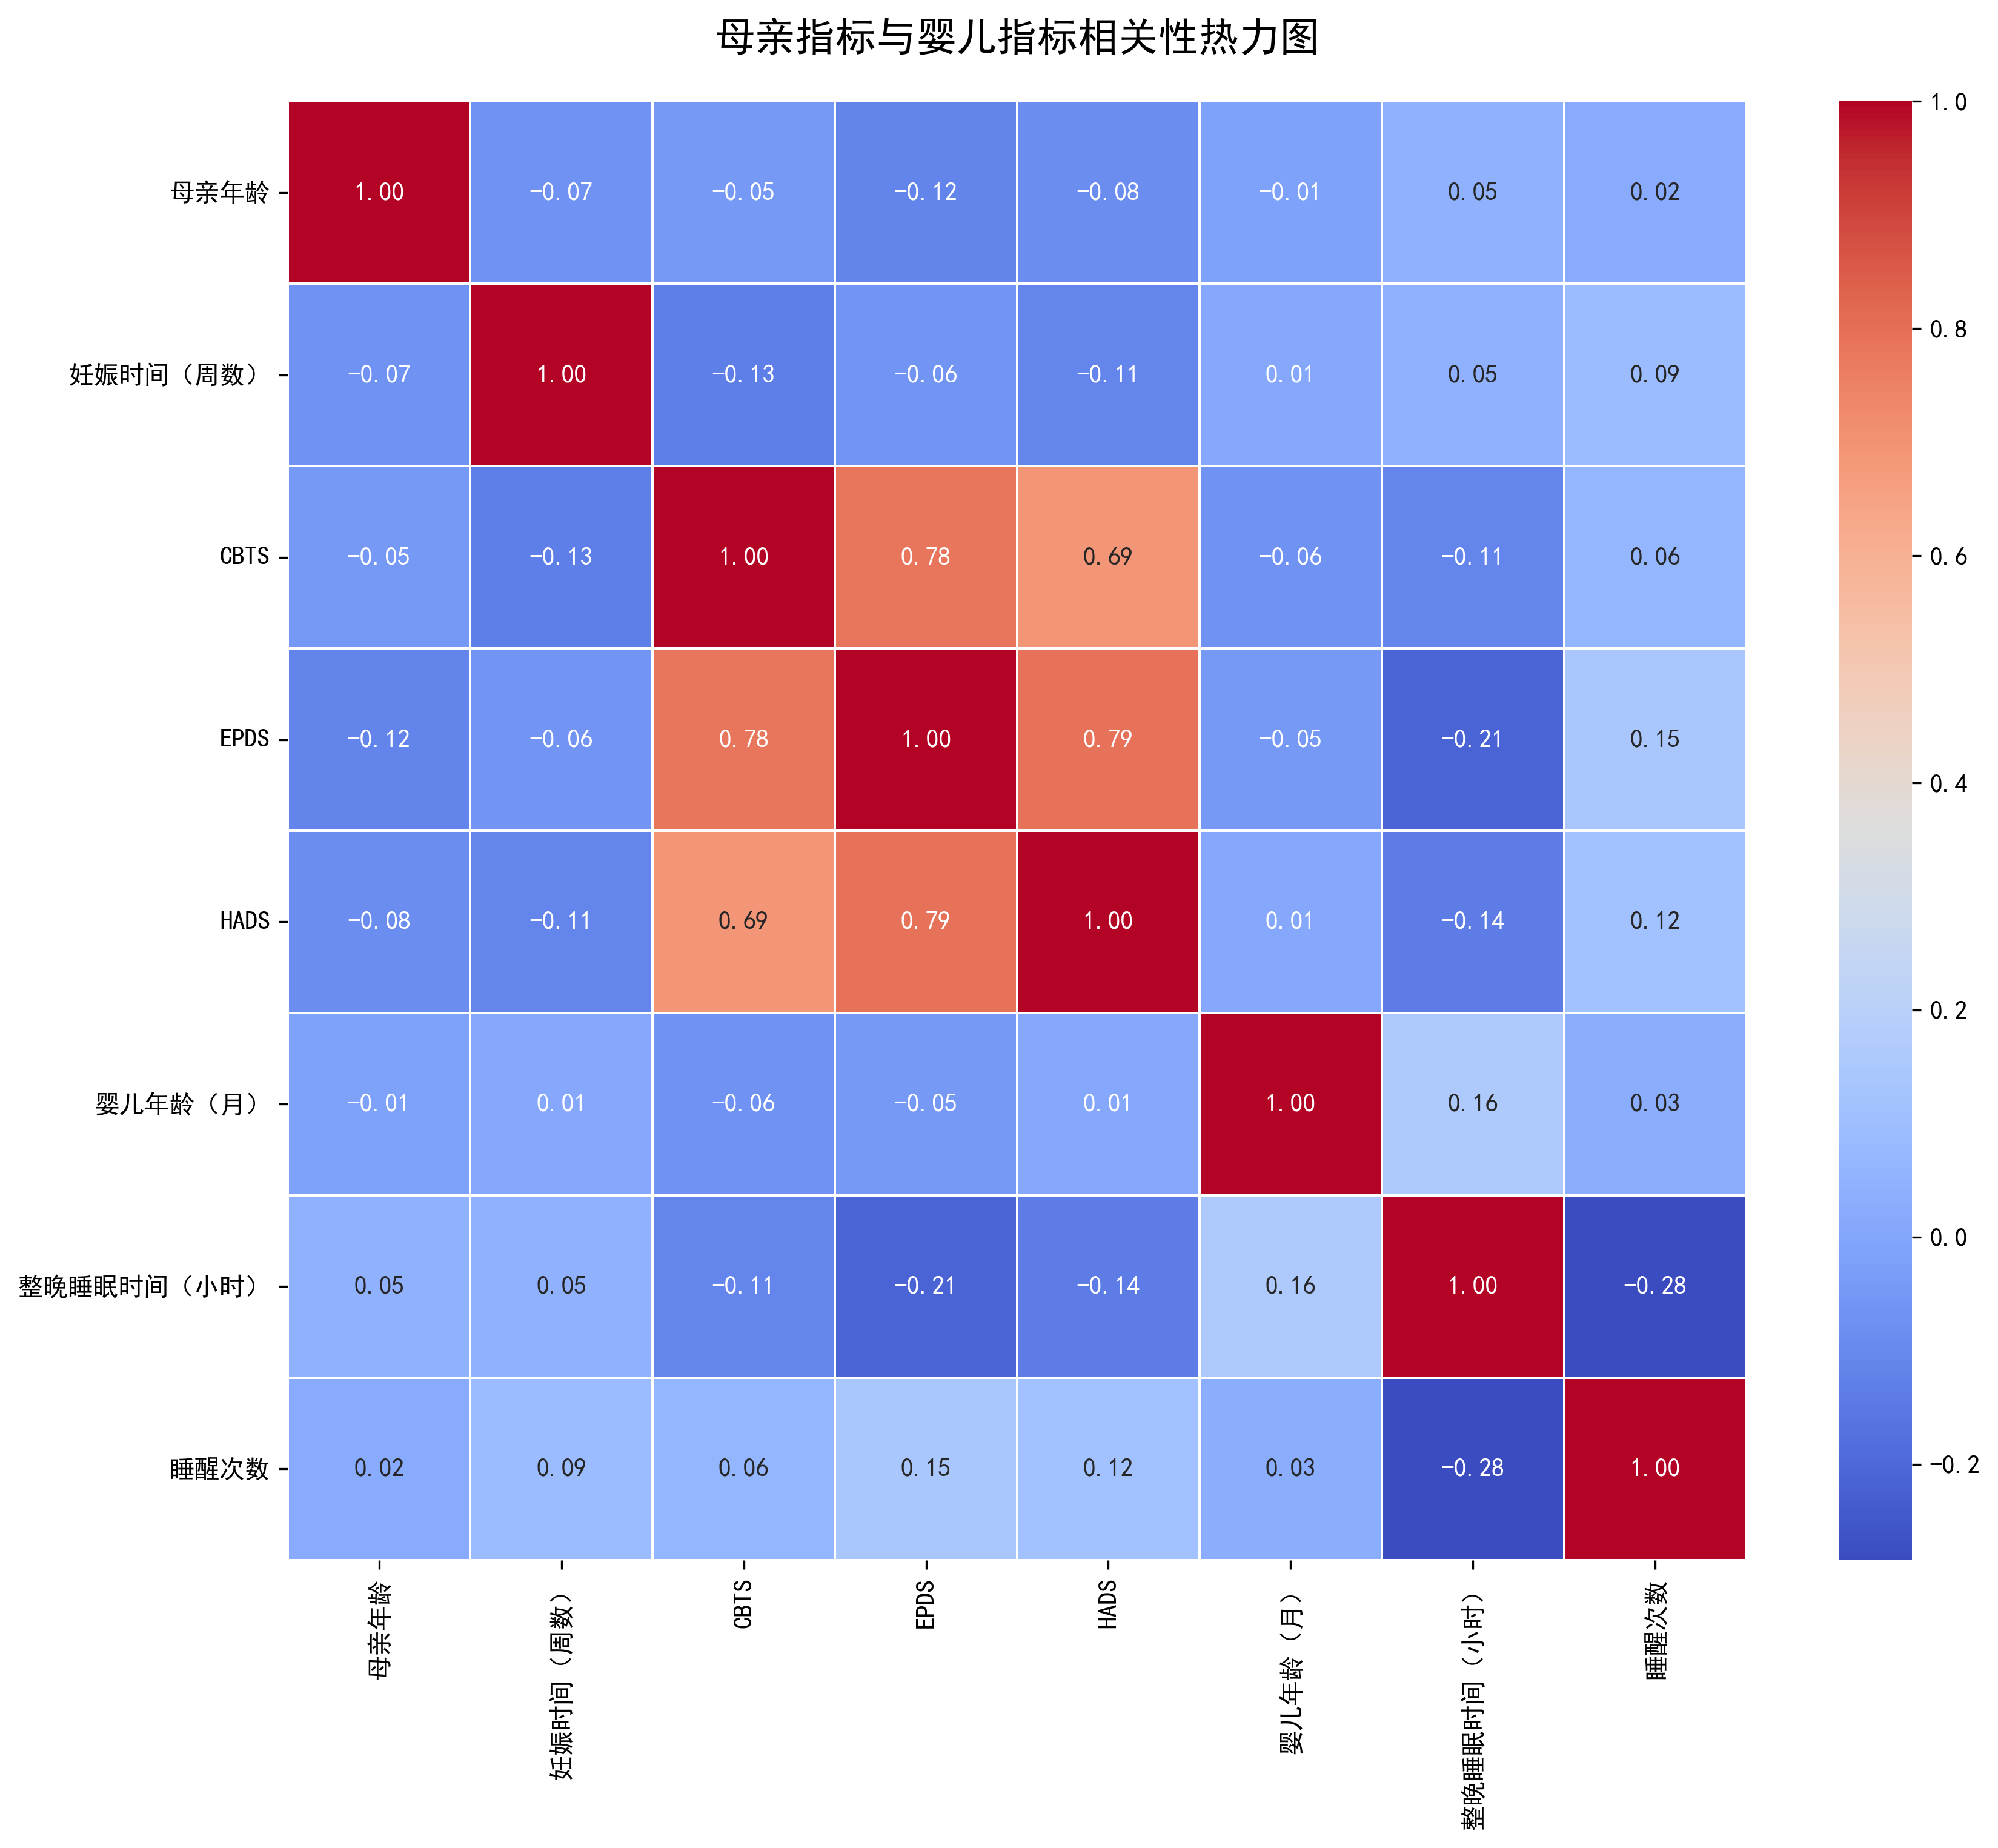
\includegraphics[width=0.8\textwidth]{figures/correlation_heatmap.png}
    \caption{母亲指标与婴儿指标相关性热力图}
    \label{fig:correlation_heatmap}
\end{figure}

\subsubsection{分类变量对连续变量的影响 (ANOVA)}
为了评估分类变量对婴儿睡眠质量指标(睡醒次数和整晚睡眠时间)的潜在影响,我们运用了方差分析(ANOVA),以检验不同类别之间是否存在显著差异。
方差分析结果强烈支持入睡方式对婴儿睡眠质量指标具有显著影响。具体而言,入睡方式对婴儿夜间睡醒次数产生了显著影响($F=16.87, p<0.001$)。如图5所示,能够自主入睡的婴儿,其夜间睡醒次数显著少于其他入睡方式的婴儿,这有力地表明自主入睡有助于提升婴儿夜间睡眠的连续性。

% 将图表移动到首次引用之后
\begin{figure}[htbp]
    \centering
    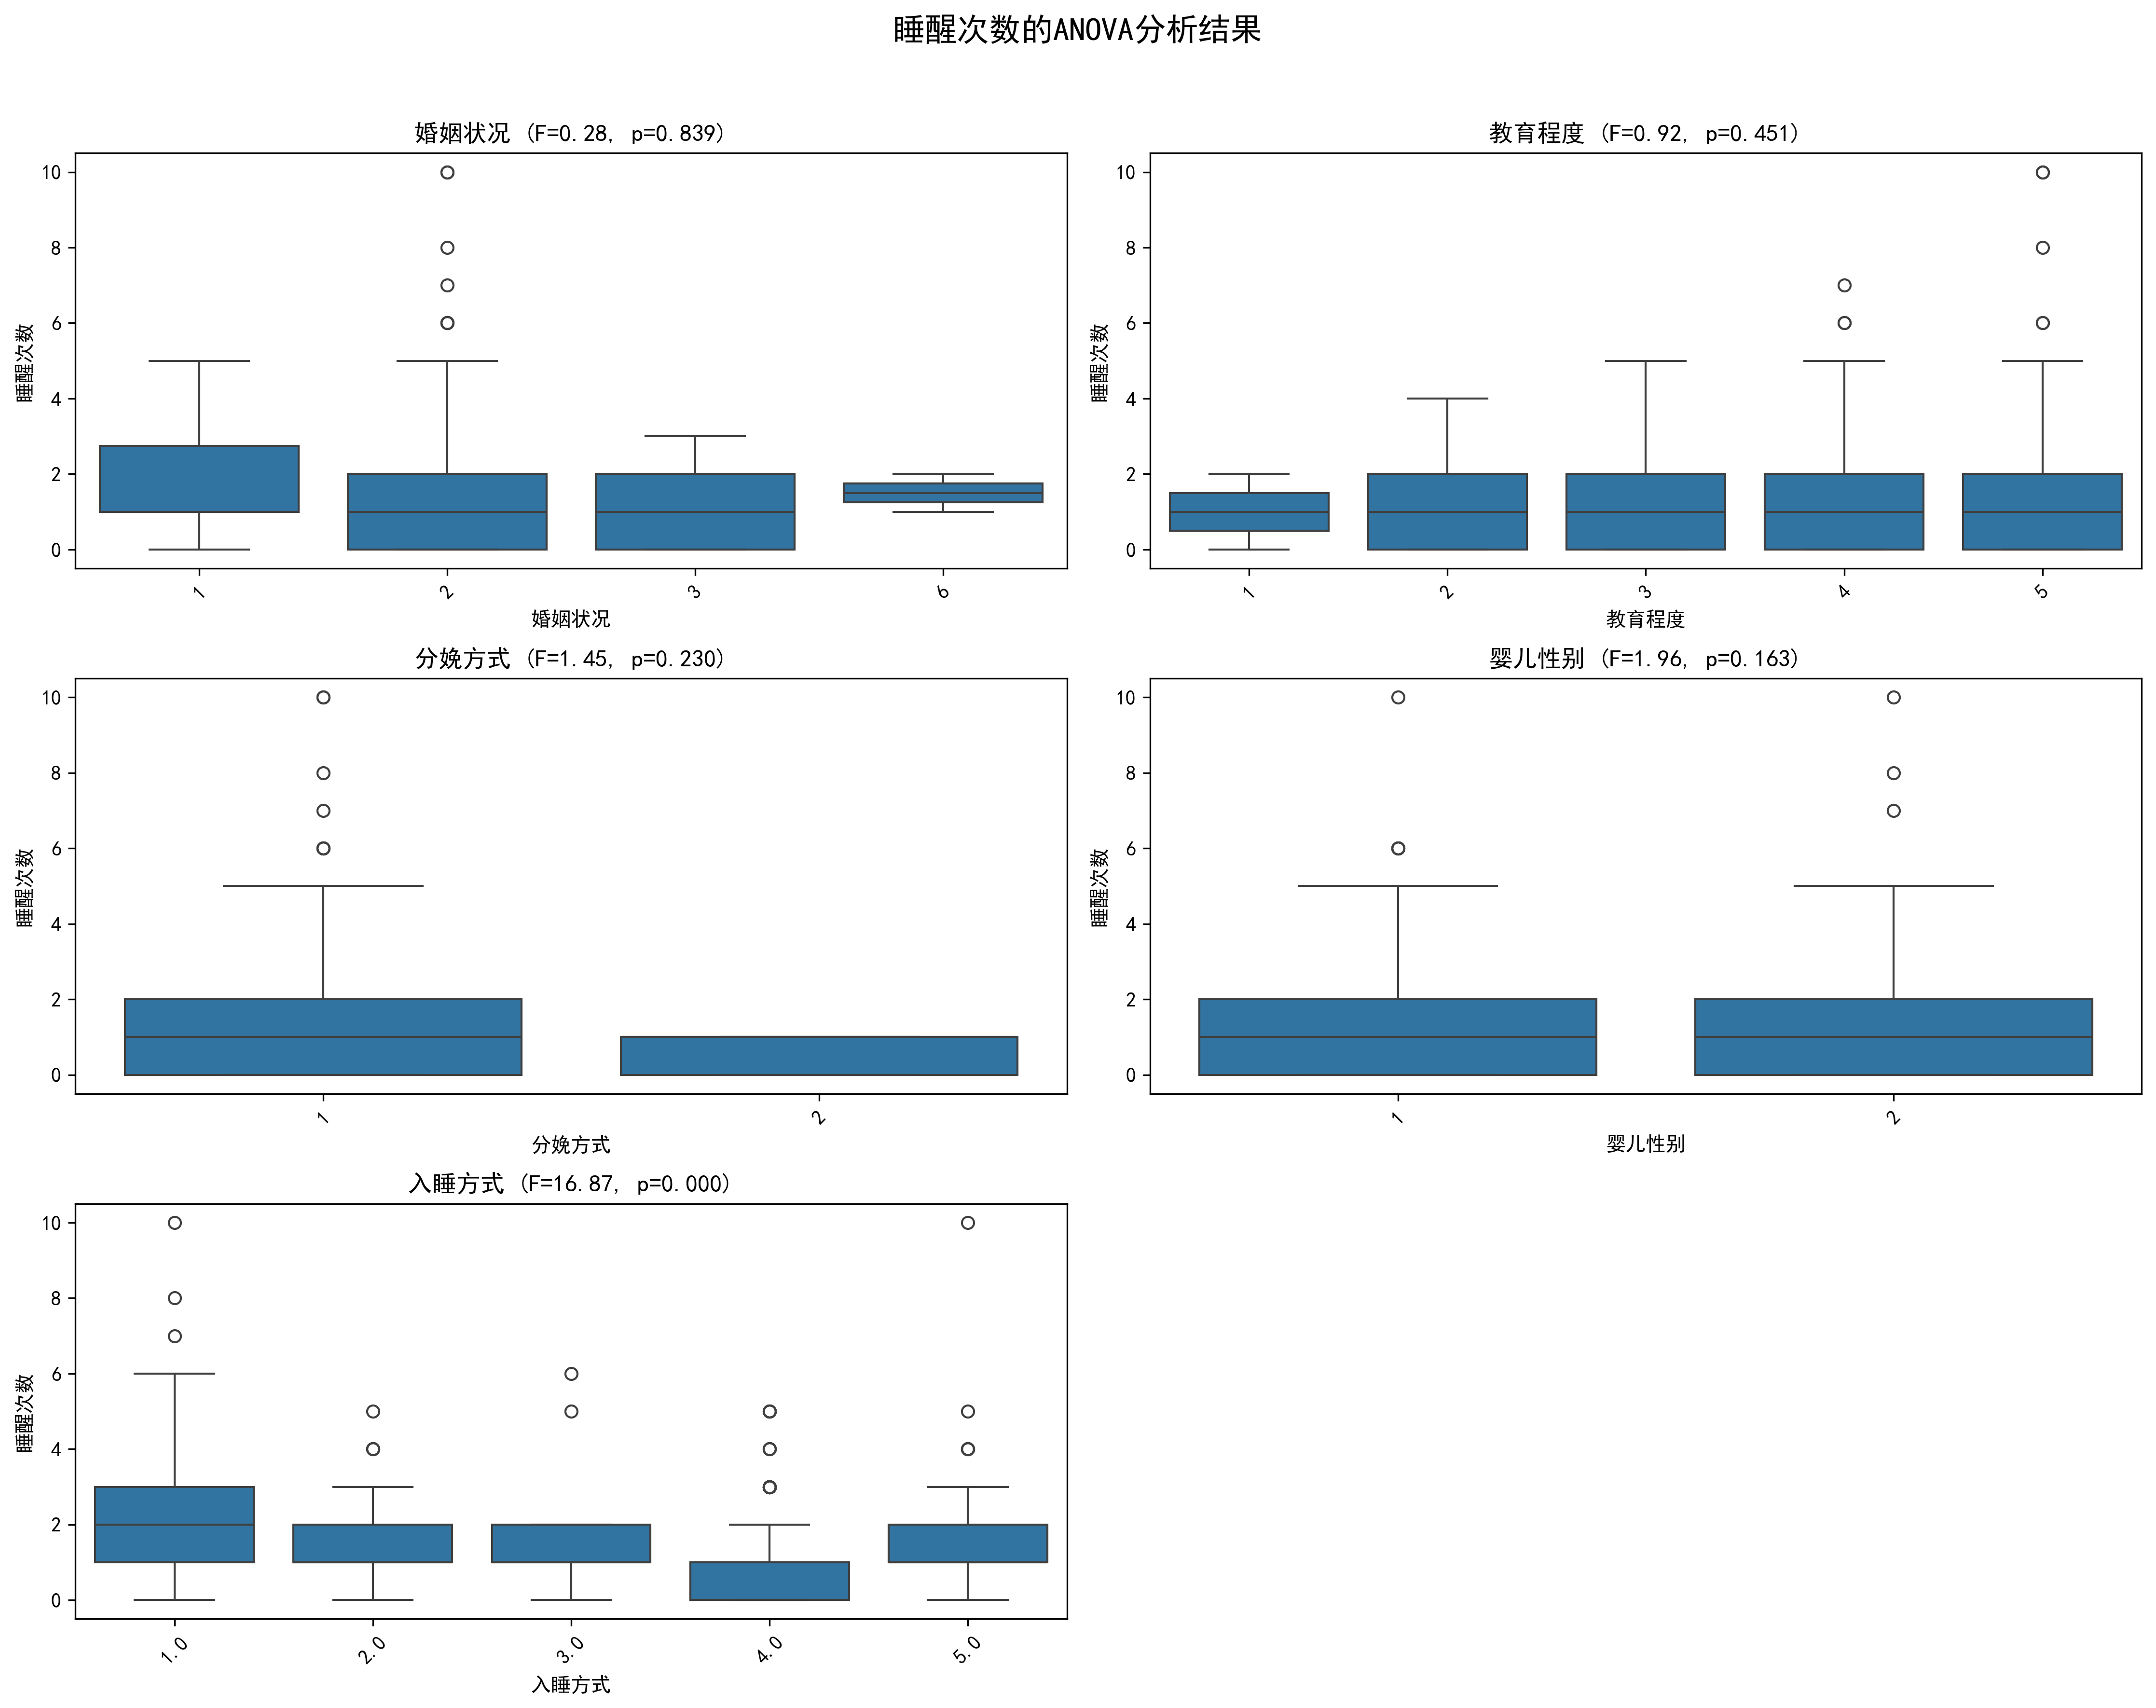
\includegraphics[width=0.9\textwidth]{figures/anova_睡醒次数_combined.png}
    \caption{睡醒次数的ANOVA分析结果}
    \label{fig:anova_wake_up_times}
\end{figure}

同样,入睡方式对婴儿的整晚睡眠时间也表现出显著影响($F=12.18, p<0.001$)。如图6所示,自主入睡的婴儿普遍拥有更长的整晚睡眠时间,进一步印证了自主入睡对提升婴儿整体睡眠质量的积极作用。

% 将图表移动到首次引用之后
\begin{figure}[htbp]
    \centering
    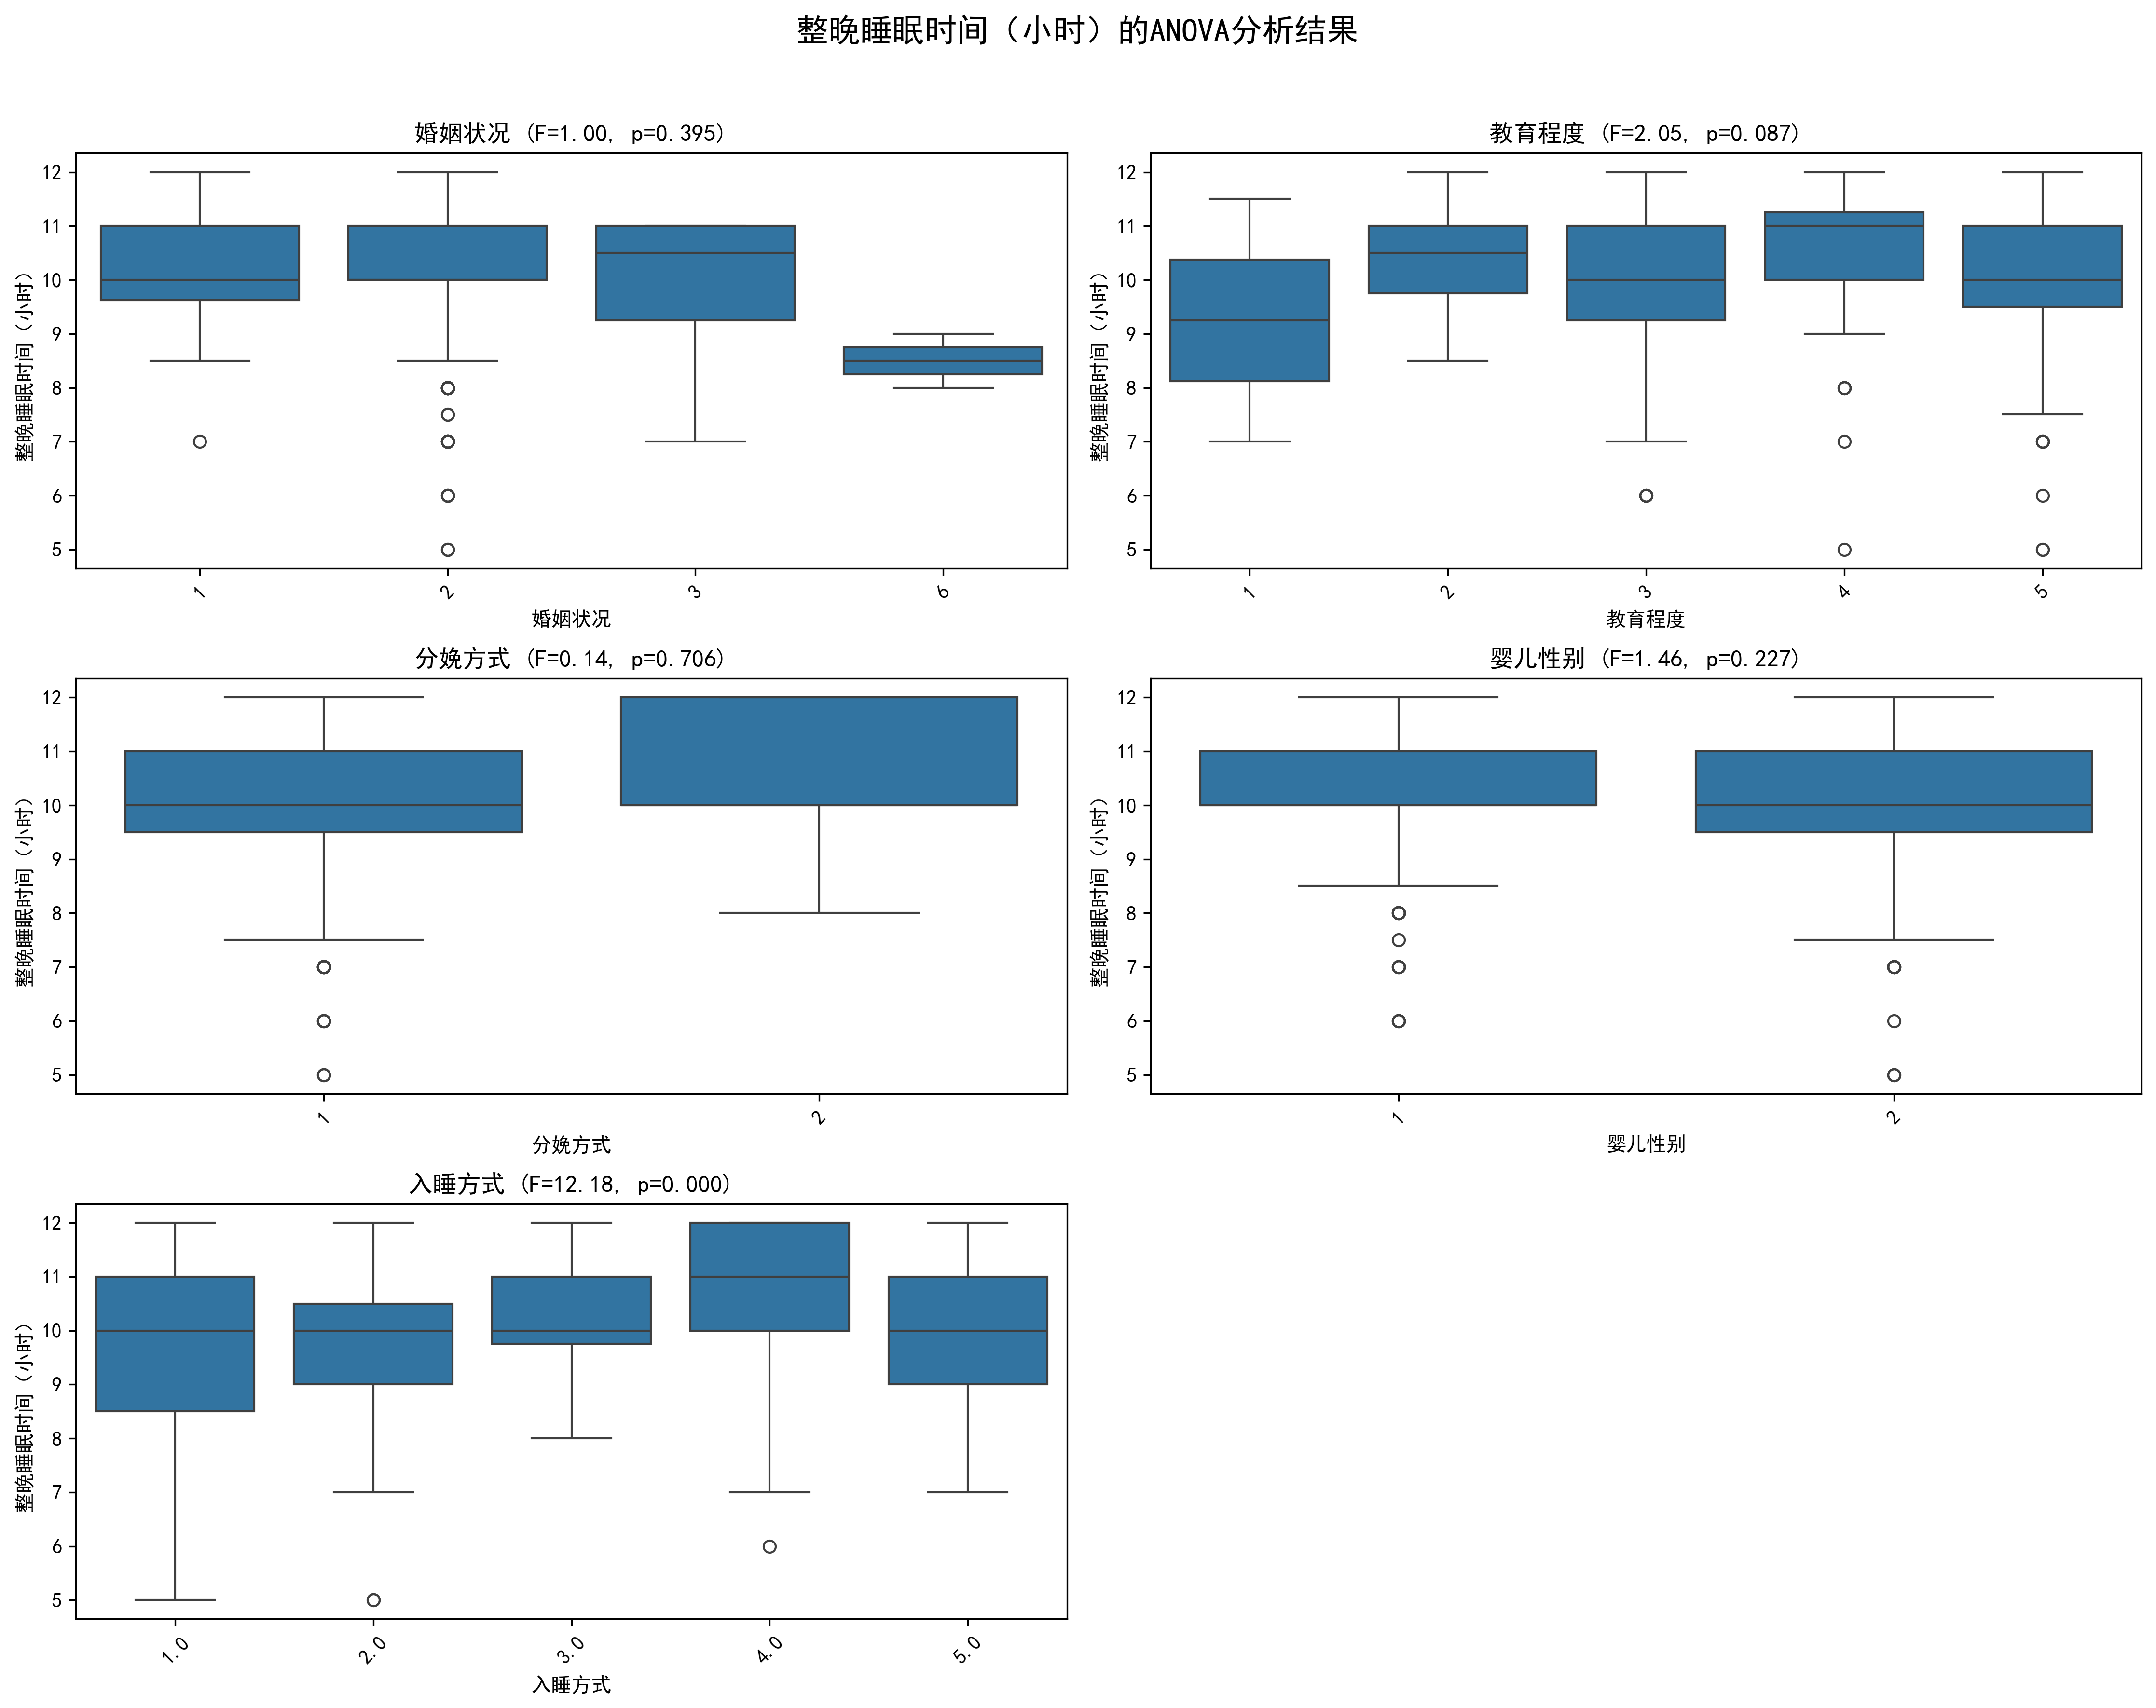
\includegraphics[width=0.9\textwidth]{figures/anova_整晚睡眠时间(小时)_combined.png}
    \caption{整晚睡眠时间(小时)的ANOVA分析结果}
    \label{fig:anova_sleep_time}
\end{figure}

值得注意的是,尽管我们考察了婚姻状况、教育程度、分娩方式以及婴儿性别等其他分类变量,但这些因素对婴儿睡眠质量的各项指标均未显示出统计学上的显著影响(所有$p>0.05$)。这可能意味着,在影响婴儿睡眠的众多因素中,这些人口学和分娩相关变量的直接作用相对较弱。

\subsubsection{分类变量间的关联性 (Chi-square)}
我们进一步采用卡方检验来探究各个分类变量之间的关联性,以识别组别间是否存在非随机的分布模式。
如图7所示,我们特别展示了那些具有统计显著性($p<0.05$)的分类变量对。卡方检验结果显示,母亲的婚姻状况与教育程度之间存在统计学上的显著关联($p=0.020$)。这提示在我们的样本中,已婚母亲的教育程度普遍高于未婚母亲,这或许反映了某些社会人口学背景下的普遍趋势。

% 将图表移动到首次引用之后
\begin{figure}[htbp]
    \centering
    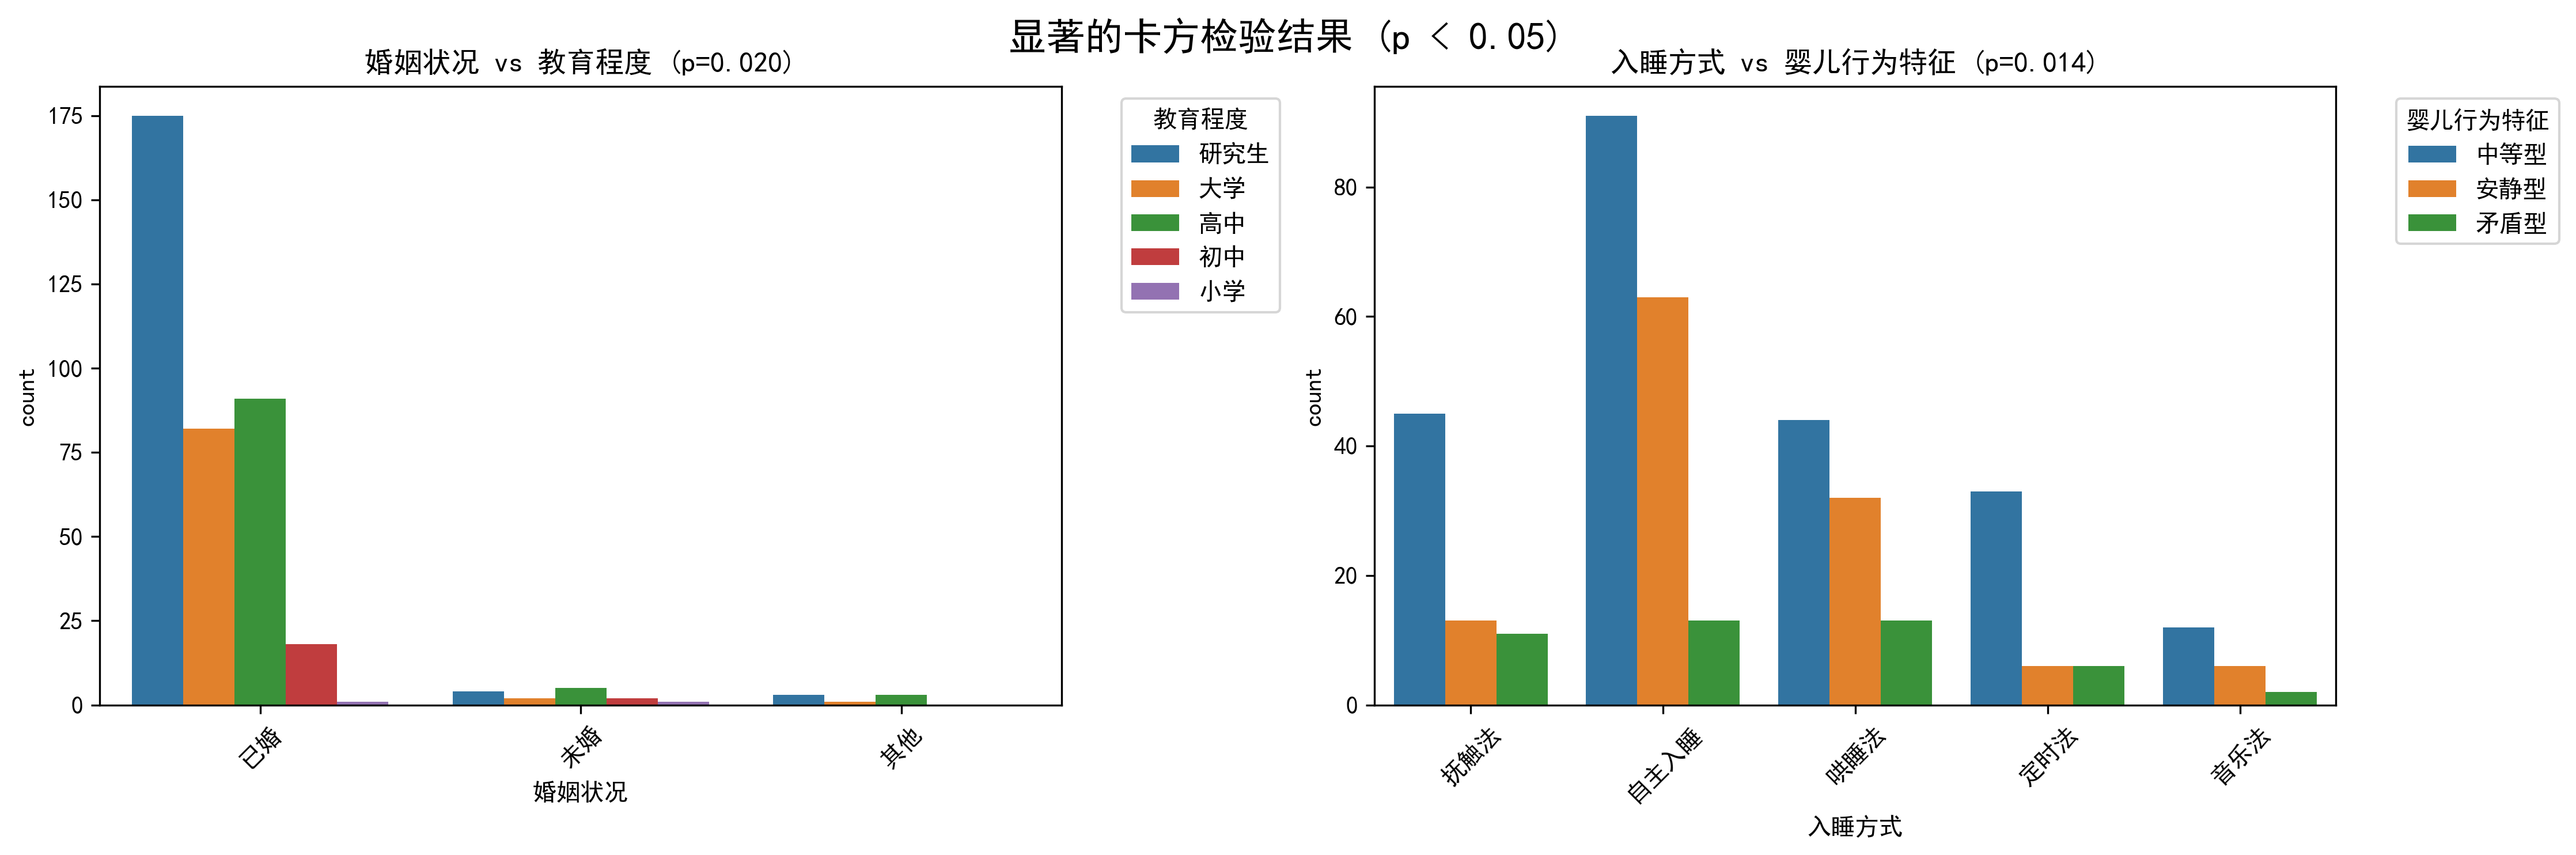
\includegraphics[width=0.9\textwidth]{figures/chi_square_significant_results.png}
    \caption{显著的卡方检验结果 ($p < 0.05$)}
    \label{fig:chi_square_significant}
\end{figure}

更为重要的发现是,入睡方式与婴儿行为特征之间存在显著关联($p=0.014$)。具体分析表明,采用自主入睡方式的婴儿,其行为模式更倾向于表现为“安静型”特征。图8则以热力图的形式呈现了所有分类变量对的p值,p值越小意味着关联性越强,进一步直观展示了这种关联。这一结果不仅强化了良好入睡习惯的重要性,也进一步揭示了其对婴儿整体行为发展所产生的积极影响。
大多数分类变量之间未检测到统计学上的显著关联,这暗示了这些因素在很大程度上是相互独立的,从而简化了后续模型中的变量选择和解释。

% 将图表移动到首次引用之后
\begin{figure}[htbp]
    \centering
    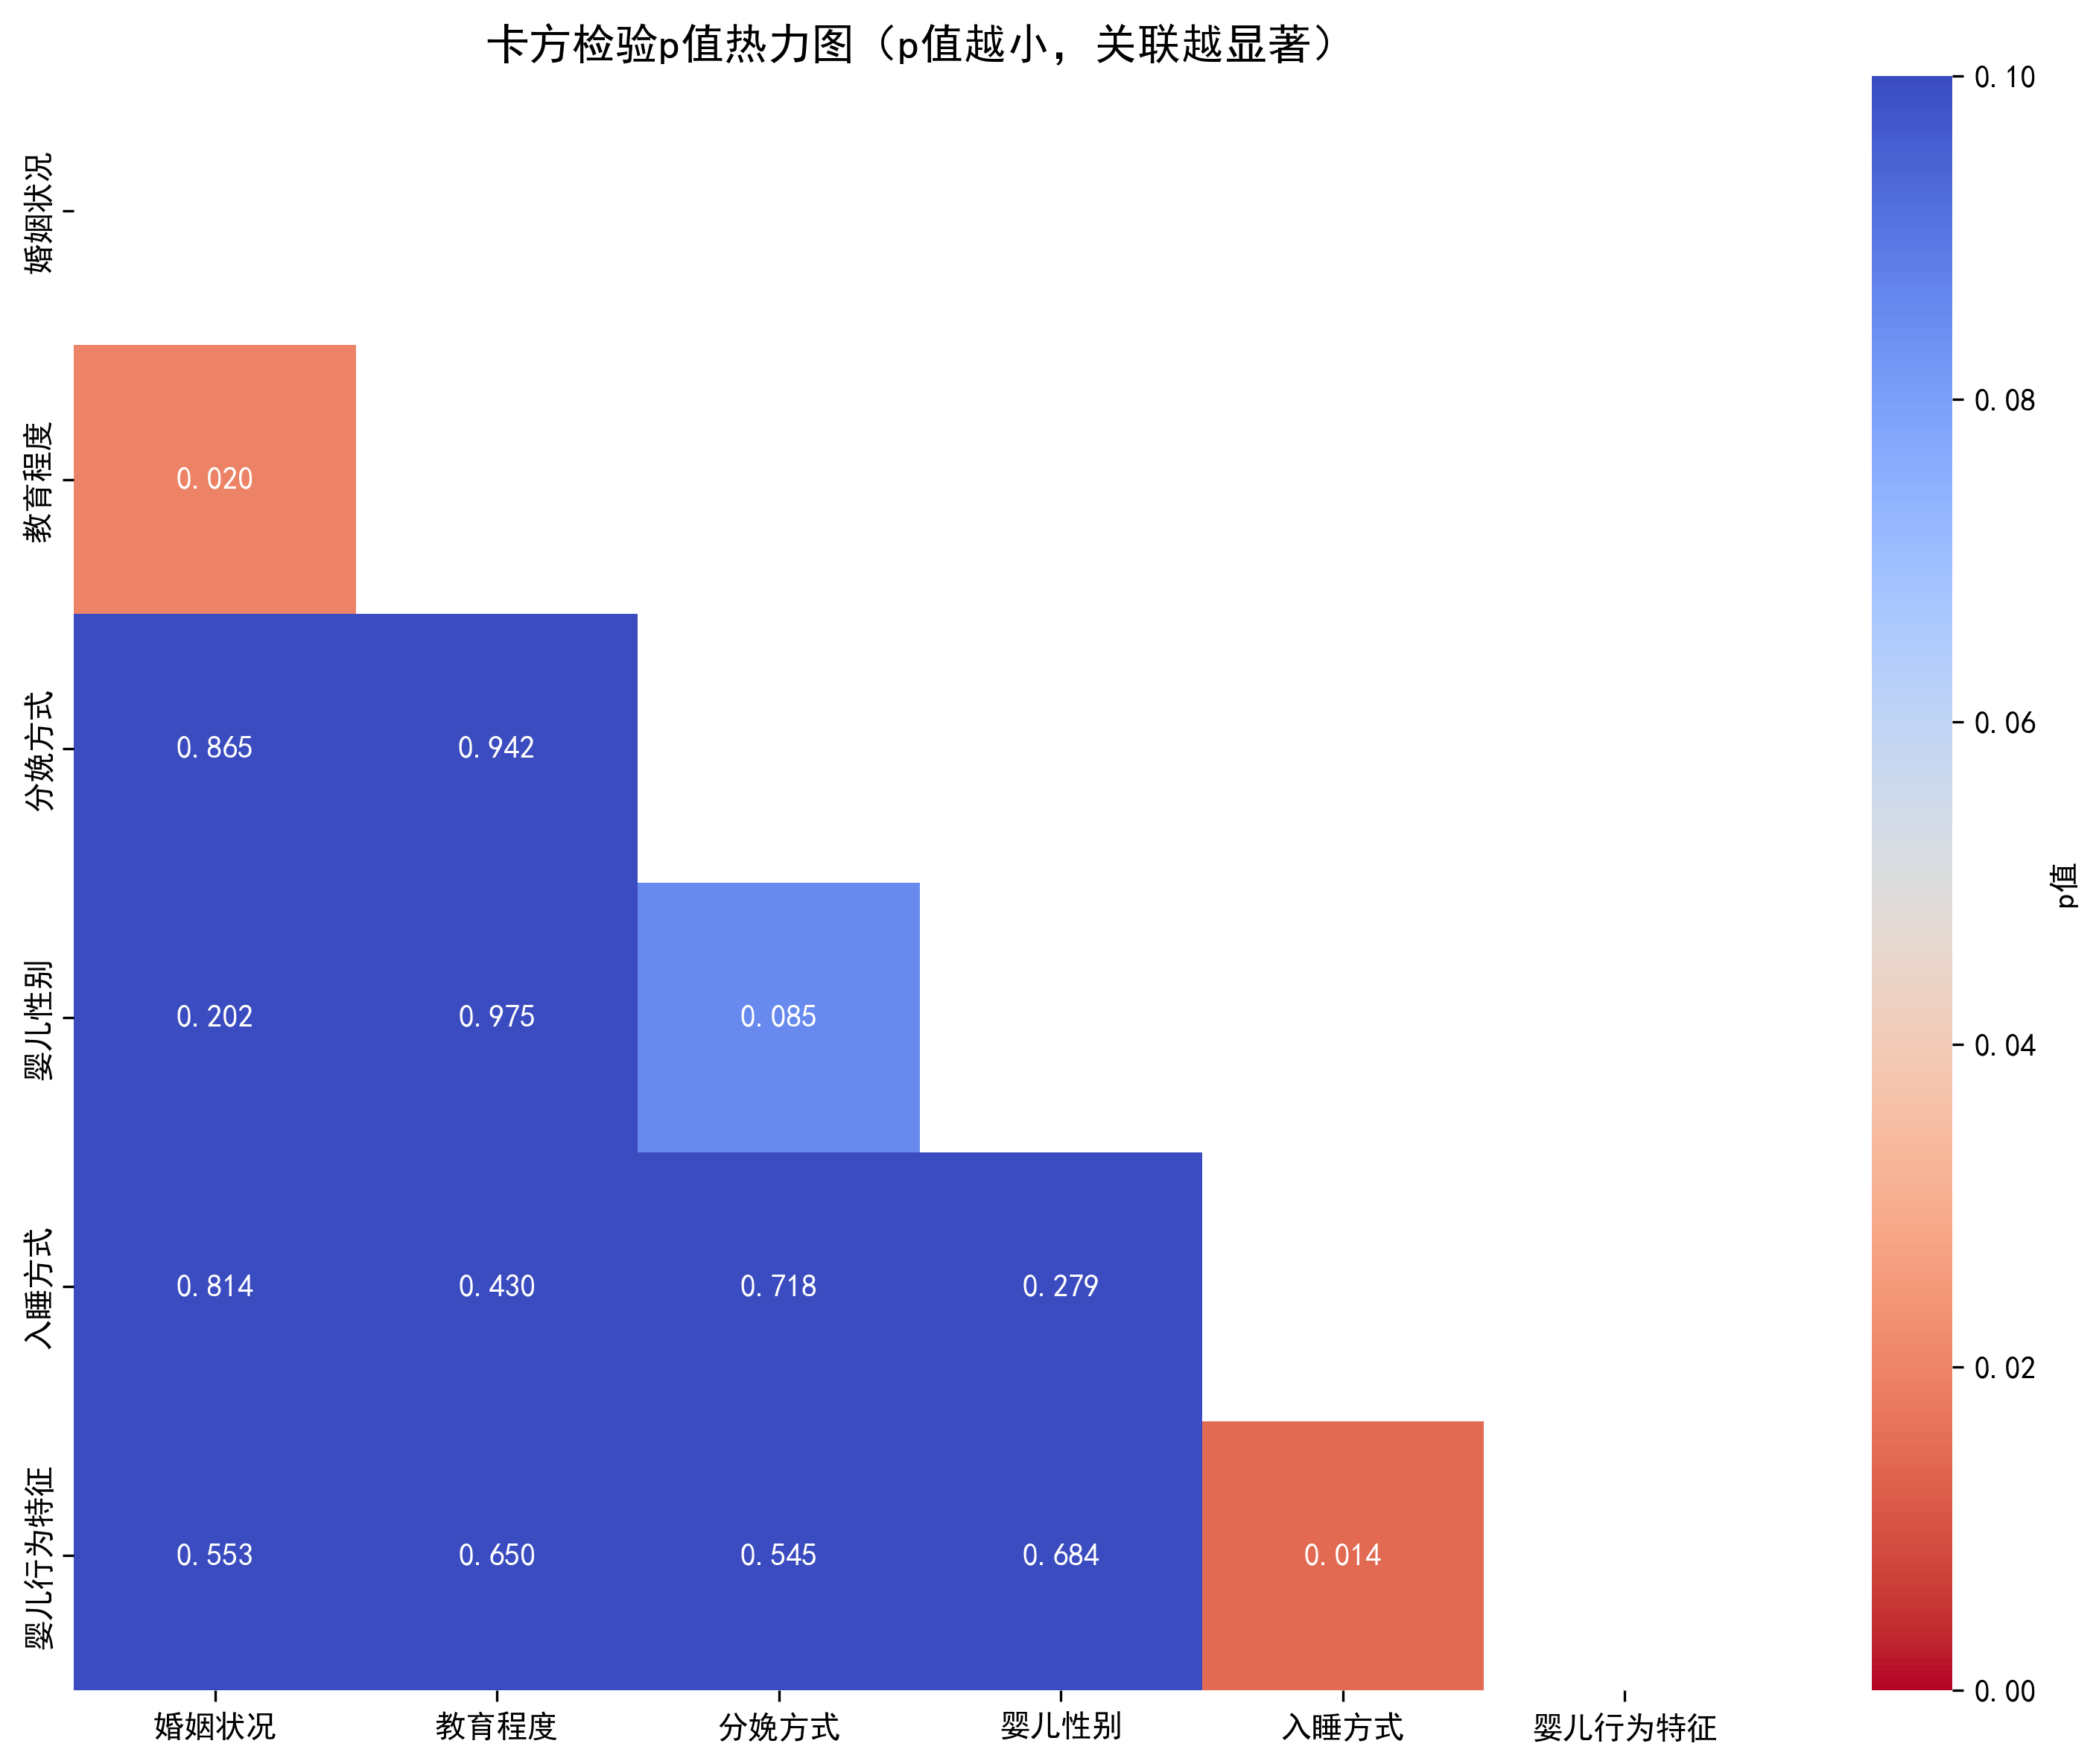
\includegraphics[width=0.6\textwidth]{figures/chi_square_p_values_heatmap.png}
    \caption{卡方检验p值热力图 (p值越小,关联越显著)}
    \label{fig:chi_square_p_values_heatmap}
\end{figure}

\subsubsection{多重共线性检查}
为了确保后续回归模型的稳健性与解释力,我们对所有数值型预测变量进行了多重共线性检查,并计算了方差膨胀因子(VIF)。VIF值能够直观反映一个自变量能否被其他自变量线性解释的程度,从而判断是否存在过度相关性。如图9所示,教育程度\_研究生的VIF值达到5.72,这是所有变量中最高的。尽管该值接近但尚未超过通常设定为10的警戒线,这表明教育程度的某些类别之间存在一定程度的共线性,但其影响仍在模型可接受的范围内。类似地,教育程度\_高中和教育程度\_大学的VIF值也相对较高,分别为4.56和4.36,进一步印证了教育背景变量内部的关联性。母亲EPDS得分的VIF值为3.94,这反映了EPDS与其他心理指标之间存在一定的相关性,与我们之前在相关性分析中的发现相符。值得庆幸的是,绝大多数预测变量的VIF值均小于2.5,这有力地表明模型中多重共线性问题得到了有效控制,预计不会对模型结果的稳定性或参数估计的准确性产生严重影响。

% 将图表移动到首次引用之后
\begin{figure}[htbp]
    \centering
    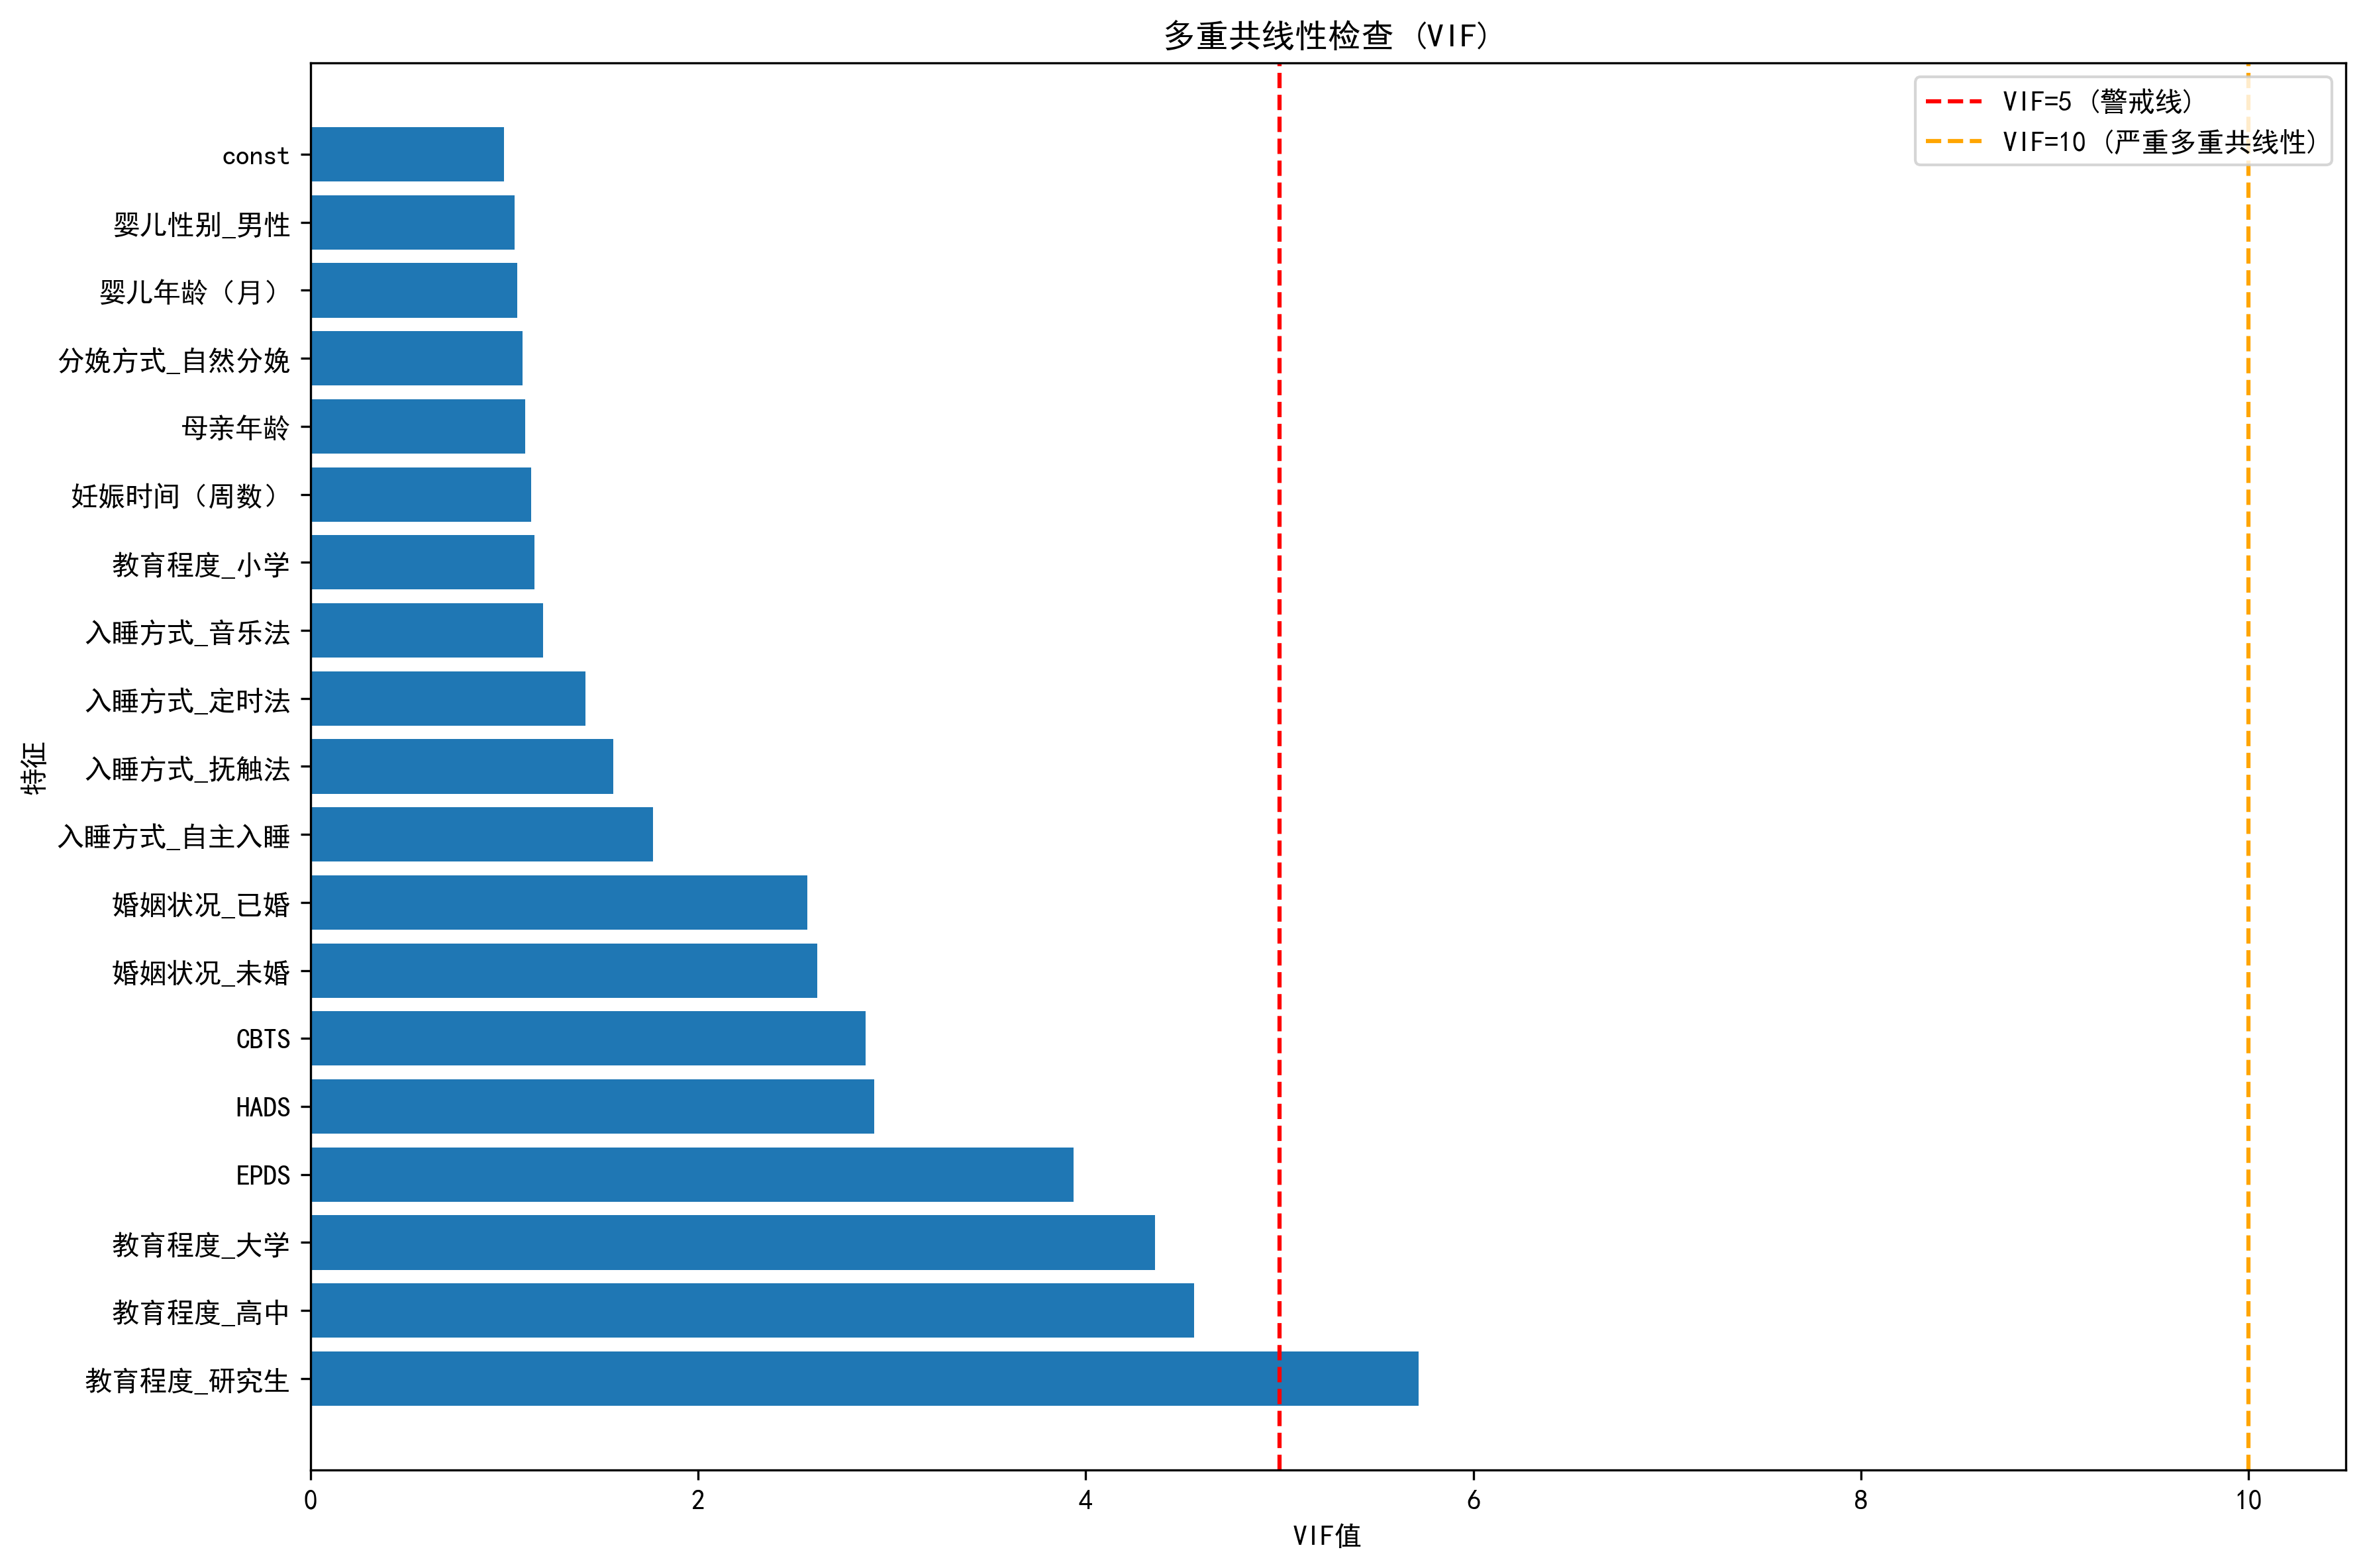
\includegraphics[width=0.7\textwidth]{figures/multicollinearity_vif.png}
    \caption{多重共线性检查 (VIF)}
    \label{fig:multicollinearity_vif}
\end{figure}

\subsection{模型选择与理论基础}
根据问题一所涉因变量的类型(连续型与多分类型),我们选择了相应的统计回归模型进行分析,以期最大化地捕捉变量间的潜在关系。

\subsubsection{婴儿睡眠质量模型:多元线性回归}
鉴于婴儿的“整晚睡眠时间”和“睡醒次数”均为连续数值型变量,我们选择多元线性回归 (Multiple Linear Regression) 作为其预测模型。多元线性回归旨在建立一个线性关系,用一个或多个自变量来预测因变量的取值,其优点在于模型简洁且易于解释。
其一般形式为:
$$ Y = \beta_0 + \beta_1 X_1 + \beta_2 X_2 + \dots + \beta_k X_k + \epsilon $$
其中:$Y$ 是因变量(如整晚睡眠时间或睡醒次数)。$X_1, X_2, \dots, X_k$ 是 $k$ 个自变量(如母亲年龄、心理指标、入睡方式等)。$\beta_0$ 是截距项。$\beta_1, \beta_2, \dots, \beta_k$ 是对应自变量的回归系数,表示在其他自变量不变的情况下,该自变量每增加一个单位,因变量的平均变化量。$\epsilon$ 是误差项,代表模型未能解释的随机变异。
模型通过最小化残差平方和(Ordinary Least Squares, OLS)来估计回归系数。模型的评估指标包括决定系数 ($R^2$)、调整决定系数 (Adjusted $R^2$)、F统计量及其p值,用于评估模型的整体拟合优度和统计显著性。

\subsubsection{婴儿行为特征模型:多项逻辑回归}
婴儿行为特征(“安静型”、“中等型”、“矛盾型”)是一个具有三个或更多无序类别的分类变量。因此,我们选择多项逻辑回归 (Multinomial Logistic Regression) 模型来分析母亲各项因素对其影响。多项逻辑回归是二元逻辑回归的自然扩展,用于预测一个多分类因变量的概率,避免了将无序类别强行排序可能引入的偏差。
它通过建立多个二元逻辑回归模型来比较每个类别与一个基准类别(参考类别)的对数发生比 (log-odds)。假设我们有 $J$ 个类别,选择第 $J$ 个类别作为参考类别。对于每个非参考类别 $j \in \{1, \dots, J-1\}$,模型估计其相对于参考类别的对数发生比:
$$ \ln\left(\frac{P(Y=j | \mathbf{X})}{P(Y=J | \mathbf{X})}\right) = \beta_{j0} + \beta_{j1} X_1 + \beta_{j2} X_2 + \dots + \beta_{jk} X_k $$
其中:$P(Y=j | \mathbf{X})$ 是在给定自变量 $\mathbf{X}$ 的情况下,因变量属于类别 $j$ 的概率。$\beta_{j}$ 是对应于类别 $j$ 的回归系数向量。发生比 (Odds Ratio, OR):$e^{\beta_{ji}}$ 表示在其他自变量不变的情况下,自变量 $X_i$ 每增加一个单位,因变量属于类别 $j$ 而而非参考类别的发生比的变化倍数。
模型的评估通常使用赤池信息准则 (AIC) 和贝叶斯信息准则 (BIC),它们平衡了模型的拟合优度和复杂度。发生比 (Odds Ratio) 的可视化是理解自变量对不同类别影响的关键,能够直观展示各因素对不同行为类型的倾向性影响。

\subsection{模型构建与求解}
在确定模型类型后,我们基于前期探索性数据分析的结果,构建并求解了各个模型,以量化母亲因素对婴儿睡眠与行为的影响。

\subsubsection{婴儿睡眠质量线性回归模型构建}
我们分别构建了预测“整晚睡眠时间”和“睡醒次数”的线性回归模型。模型中纳入了所有经过预处理的母亲身体指标、心理指标以及独热编码后的分类变量。

\paragraph{整晚睡眠时间模型}
该睡眠时间模型在统计学上整体显著($F=4.66, p < 0.001$),这表明模型中的自变量组合能够对婴儿的整晚睡眠时间产生显著影响。然而,模型的解释力相对有限,其决定系数$R^2$为0.184,调整决定系数$Adjusted~R^2$为0.145。这提示虽然模型捕捉到了一部分变异,但婴儿睡眠时间的影响因素可能更为复杂多样,现有变量仅能解释约18.4\%的变异,可能存在更多未被纳入的生理或环境因素。
在显著预测因子方面,入睡方式中的“自主入睡”表现出最为显著的正向影响。这意味着,与其他入睡方式相比,能够自主入睡的婴儿普遍拥有显著更长的整晚睡眠时间。这一发现不仅再次验证了前期探索性数据分析(ANOVA)的结论,更强调了培养婴儿自主入睡能力对提升其睡眠质量具有决定性的作用。此外,母亲的EPDS(爱丁堡产后抑郁量表)得分与婴儿整晚睡眠时间呈现显著的负相关关系。具体而言,母亲的EPDS得分越高,其婴儿的整晚睡眠时间则越短。这一结果清晰地揭示了母亲抑郁情绪对婴儿睡眠模式的负面影响,从而提示了心理干预的必要性。

\paragraph{睡醒次数模型}
与睡眠时间模型类似,睡醒次数模型在统计上整体显著($F=5.32, p < 0.001$),且其解释力略高于睡眠时间模型($R^2 = 0.205$, Adjusted $R^2 = 0.167$)。
在显著预测因子方面,如同在睡眠时间模型中,入睡方式在此模型中依然是影响婴儿夜间睡醒次数最为显著的因素。具体分析显示,自主入睡的婴儿夜间睡醒次数明显更少,进一步强调了其对改善婴儿睡眠连续性的积极作用,并为育儿指导提供了明确方向。此外,母亲的HADS(医院焦虑抑郁量表)得分与婴儿夜间睡醒次数呈现显著的正相关关系。这意味着母亲的焦虑抑郁程度越高,婴儿夜间睡醒的次数越多。这一结果有力地印证了母亲心理健康状况与婴儿睡眠质量之间的紧密联系,提示了心理压力对婴儿睡眠节律的干扰。

\subsubsection{婴儿行为特征多项逻辑回归模型构建}
考虑到婴儿行为特征(“安静型”、“中等型”、“矛盾型”)属于无序多分类变量,我们构建了多项逻辑回归模型以探究母亲各项因素对其影响。在此模型中,我们选择将“中等型”婴儿作为参考类别,进而分析其他两类(“安静型”和“矛盾型”)相对于“中等型”的对数发生比。
模型的评估指标分别为$AIC = 693.31$和$BIC = 844.02$。尽管模型能够有效区分不同的行为特征类型,但其预测准确率仍存在进一步优化的空间。
在显著预测因子与发生比分析方面,模型结果显示,CBTS、EPDS和HADS这三项母亲心理健康指标对婴儿行为特征具有显著的影响力。具体而言,当母亲的心理压力越大,即CBTS、EPDS和HADS得分越高时,其婴儿表现为“矛盾型”行为特征的可能性相对于“中等型”婴儿显著增加。这一发现强烈提示,母亲的心理健康问题可能直接导致或加剧婴儿出现更具挑战性的行为模式。
入睡方式被证实是影响婴儿行为特征的另一个关键因素。相较于“中等型”婴儿,采用“自主入睡”方式的婴儿更倾向于表现为“安静型”行为特征。这进一步强调了培养良好入睡习惯的重要性,更揭示了其在塑造婴儿积极行为模式方面的潜在作用。
母亲的教育程度对婴儿行为特征也展现出一定的影响。通常观察到,教育程度越高的母亲,其婴儿表现出“安静型”行为特征的可能性越大。这可能间接反映了较高教育程度的母亲在育儿理念、家庭环境创设或早期干预策略上的优势,从而有利于培养婴儿的稳定行为模式。
图10直观展示了各预测变量对婴儿行为特征影响的发生比,为上述分析提供了可视化证据。

% 将图表移动到首次引用之后
\begin{figure}[htbp]
    \centering
    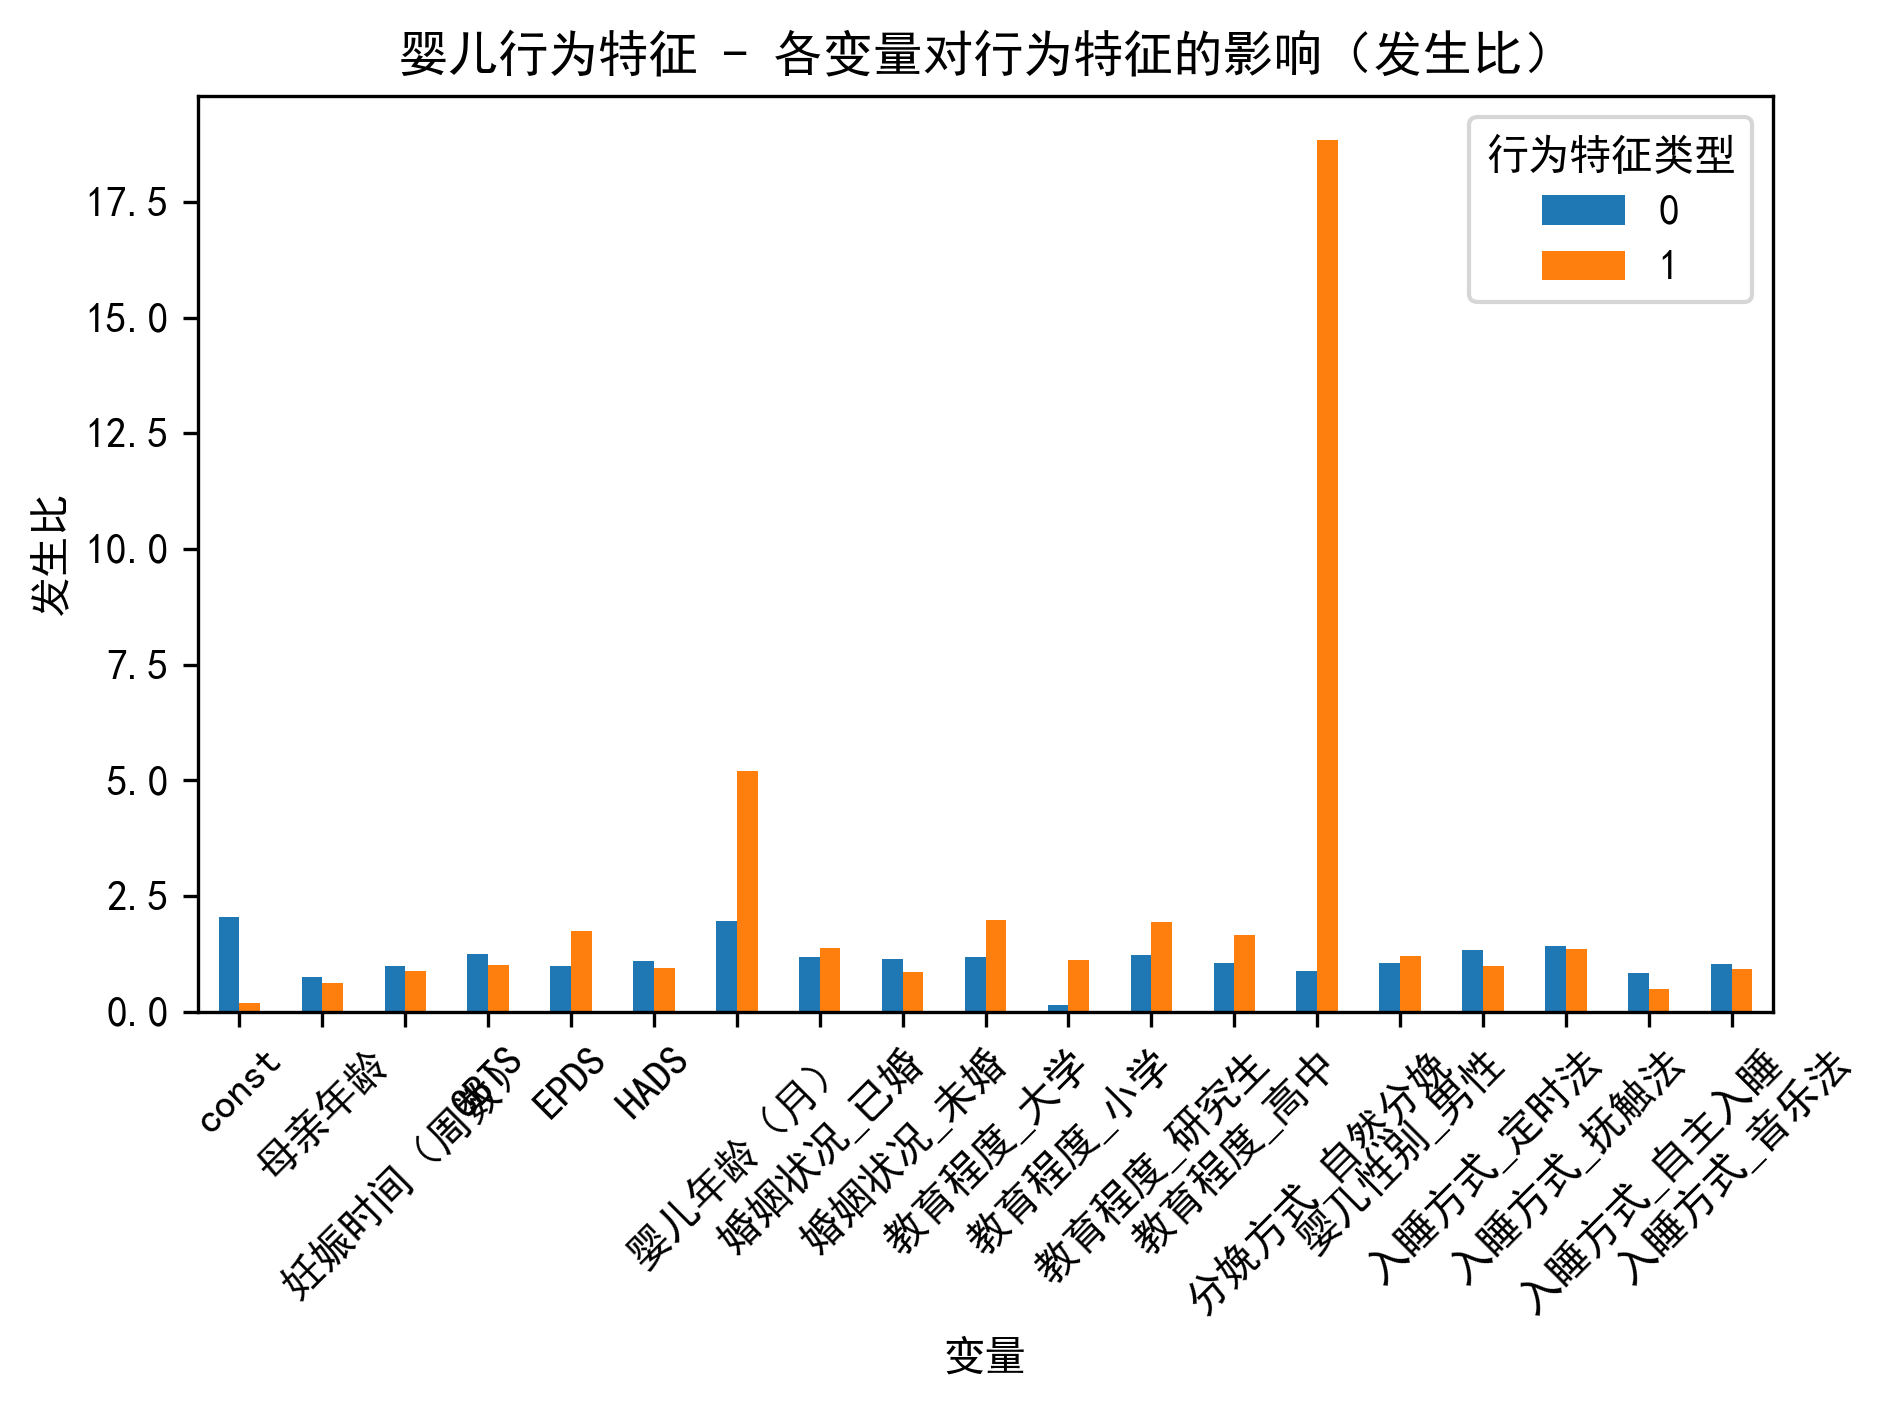
\includegraphics[width=0.8\textwidth]{figures/婴儿行为特征_odds_ratios.png} % 假设此图片文件也可用
    \caption{婴儿行为特征发生比可视化}
    \label{fig:baby_behavior_odds_ratios}
\end{figure}

\subsection{模型结果与分析}
综合上述多元线性回归与多项逻辑回归模型的分析结果,我们得以深入剖析母亲身心健康与婴儿早期发展之间的复杂关系,并得出以下关键发现:

本研究构建的模型一致揭示,母亲的抑郁情绪(EPDS)、焦虑水平(HADS)以及分娩相关创伤后应激(CBTS)症状与婴儿的睡眠质量及行为特征之间存在显著且不容忽视的关联。具体而言,母亲所承受的心理压力越大,其婴儿的整晚睡眠时间越短,夜间睡醒次数越多,并且其行为模式也越倾向于表现出“矛盾型”特征。这一核心发现有力地强调了在产妇保健体系中,将心理健康筛查与早期干预纳入常规服务的重要性,以积极促进婴儿的全面健康发展。

无论是婴儿的整晚睡眠时间、夜间睡醒次数的分析中,还是在婴儿行为特征的预测模型里,入睡方式均被反复确认为最关键的影响因素之一。研究结果清晰表明,那些能够自主入睡的婴儿普遍拥有更长的整晚睡眠时间、更少的夜间睡醒次数,并且其行为模式更倾向于表现为“安静型”特征。这不仅为日常育儿实践提供了明确且具有操作性的指导,更凸显了积极引导和培养婴儿自主入睡能力在改善其睡眠质量和促进其良好行为模式发展方面的核心价值。

尽管本研究构建的模型在统计学上均达到了显著水平,但多元线性回归模型所能解释的婴儿睡眠质量变异比例($R^2$值约为0.18至0.20)相对有限。这提示我们,婴儿的睡眠和行为发展是一个极其复杂的生物-心理-社会交互过程,除了本模型所纳入的母亲身心健康状态和育儿方式等可量化因素外,很可能还存在大量未被模型捕捉或量化的遗传因素、环境影响、生理机制或其他社会经济因素,这些未纳入的因素共同作用,导致了婴儿发展中显著的个体差异。因此,在实际的临床干预和育儿指导中,必须充分考虑个体的特异性,并提供多维度、个性化的支持方案。

母亲的CBTS、EPDS和HADS得分之间表现出高度的相关性,这强烈暗示了这些心理困扰并非孤立存在,而是倾向于相互关联并同时出现的综合性问题。在多项逻辑回归模型中,这些心理指标共同作用于婴儿的行为特征,进一步凸显了它们对婴儿发展模式的综合性影响。这一发现进一步强调了在临床实践中,对产妇心理健康的干预应采取更为综合、整体性的策略,而非仅仅针对单一症状进行碎片化处理,以期达到更全面的积极效果。



\section{问题二的模型的建立和求解}
\subsection{模型建立}

引用\cref{fig:双图},引用\cref{fig:双图a},引用\cref{fig:双图b}。

\begin{figure}[ht]
\centering
\subcaptionbox{双图a子标题\label{fig:双图a}}
{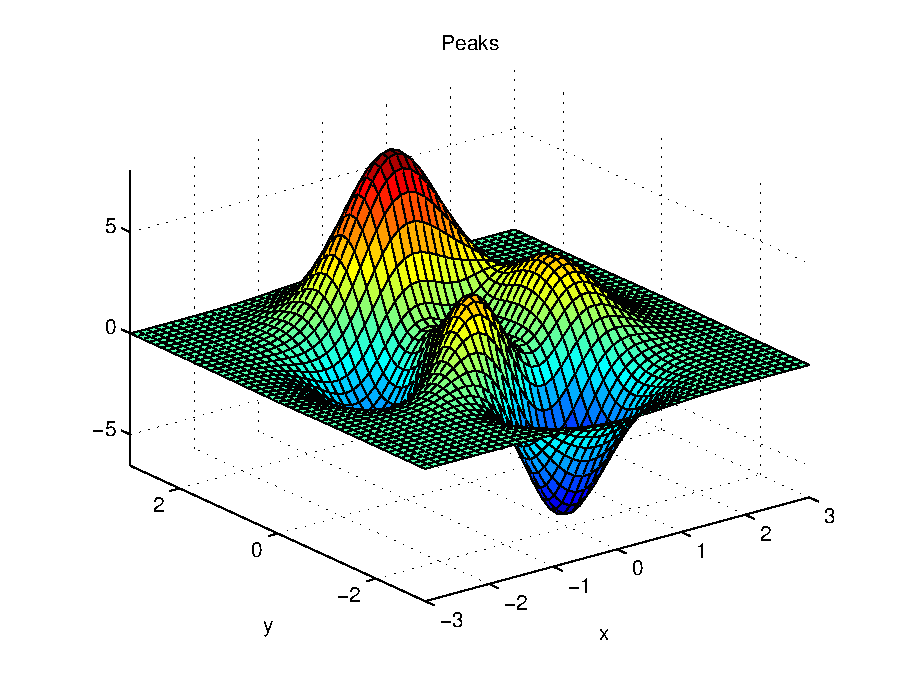
\includegraphics[width=.4\textwidth]{example.eps}}
\subcaptionbox{双图b子标题\label{fig:双图b}}
{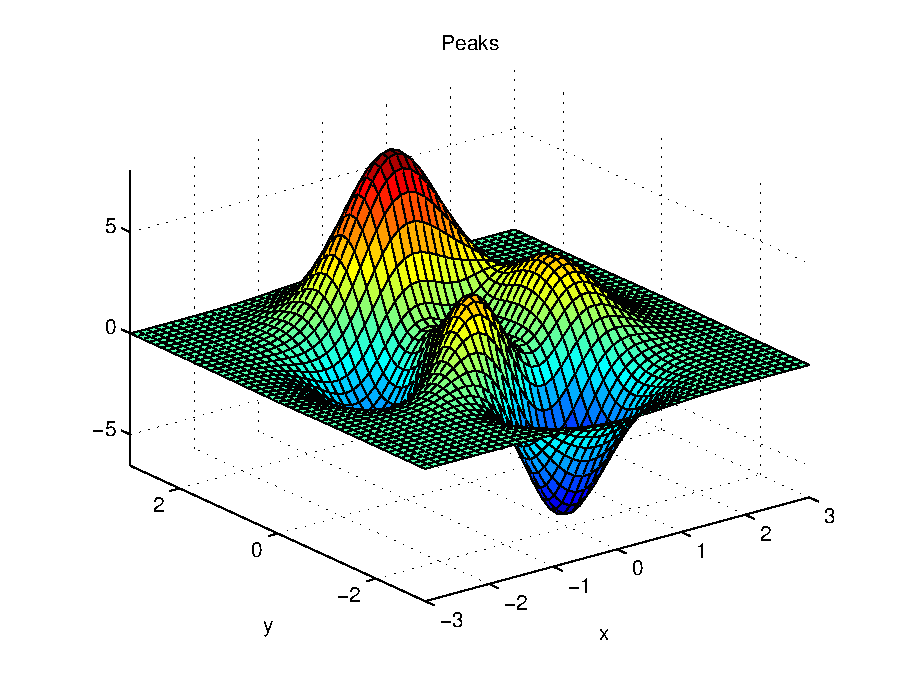
\includegraphics[width=.4\textwidth]{example.eps}}
\caption{双图}\label{fig:双图}
\end{figure} 

\subsection{模型求解}

\textbf{Step1:} 

\textbf{Step2:} 

\textbf{Step3:} 

\subsection{求解结果}

%%%%%%%%%%%%%%%%%%%%%%%%%%%%%%%%%%%%%%%%%%%%%%%%%%%%%%%%%%%%% 

\section{问题三的模型的建立和求解}
\subsection{模型建立}

\subsection{模型求解}

\textbf{Step1:} 

\textbf{Step2:} 

\textbf{Step3:} 

\subsection{求解结果}

%%%%%%%%%%%%%%%%%%%%%%%%%%%%%%%%%%%%%%%%%%%%%%%%%%%%%%%%%%%%% 

\section{问题四的模型的建立和求解}
\subsection{模型建立}

\subsection{模型求解}

\textbf{Step1:} 

\textbf{Step2:} 

\textbf{Step3:} 

\subsection{求解结果}

%%%%%%%%%%%%%%%%%%%%%%%%%%%%%%%%%%%%%%%%%%%%%%%%%%%%%%%%%%%%%

\section{模型的分析与检验}

\subsection{灵敏度分析}

\subsection{误差分析}

%%%%%%%%%%%%%%%%%%%%%%%%%%%%%%%%%%%%%%%%%%%%%%%%%%%%%%%%%%%%%

\section{模型的评价}

\subsection{模型的优点}
\begin{itemize}[itemindent=2em]
\item 优点1
\item 优点2
\item 优点3
\end{itemize}

\subsection{模型的缺点}
\begin{itemize}[itemindent=2em]
\item 缺点1
\item 缺点2
\end{itemize}

%%%%%%%%%%%%%%%%%%%%%%%%%%%%%%%%%%%%%%%%%%%%%%%%%%%%%%%%%%%%%
%% 参考文献
\nocite{*}
\bibliographystyle{gbt7714-numerical}  % 引用格式
\bibliography{ref.bib}  % bib源

\newpage
%%%%%%%%%%%%%%%%%%%%%%%%%%%%%%%%%%%%%%%%%%%%%%%%%%%%%%%%%%%%%
%% 附录
\begin{appendices}
\section{文件列表}
\begin{table}[H]
\centering
\begin{tabularx}{\textwidth}{LL}
\toprule
文件名   & 功能描述 \\
\midrule
q1.m & 问题一程序代码 \\
q2.py & 问题二程序代码 \\
q3.c & 问题三程序代码 \\
q4.cpp & 问题四程序代码 \\
\bottomrule
\end{tabularx}
\label{tab:文件列表}
\end{table}

\section{代码}
\noindent q1.m
\lstinputlisting[language=matlab]{code/q1.m}
q2.py
\lstinputlisting[language=python]{code/q2.py}
q3.c
\lstinputlisting[language=c]{code/q3.c}
q4.cpp
\lstinputlisting[language=c++]{code/q4.cpp}
\end{appendices}
\end{document}


%%%%%双图模板%%%%%%
\begin{figure}
\centering
\subcaptionbox{炉温曲线示意图\label{fig:双图a}}
{\includegraphics[width=.4\textwidth]{炉温曲线示意图.png}}
\subcaptionbox{问题1炉温曲线\label{fig:双图b}}
{\includegraphics[width=.4\textwidth]{问题1炉温曲线.png}}
\caption{双图}\label{fig:双图}
\end{figure} 
%%%%%双图模板%%%%%%